\documentclass[14pt]{extarticle}
\usepackage[T1]{fontenc}
\usepackage[default]{sourcesanspro}
\usepackage[letterpaper,top=0.75in,bottom=0.75in,left=0.65in,right=0.65in,
  headheight=18pt,headsep=0.28in,footskip=0.45in]{geometry}
\usepackage{tikz}
\usepackage{fancyhdr}
\usepackage[none]{hyphenat}
\usepackage{ragged2e}
\definecolor{cube}{RGB}{176,204,236}
\definecolor{folder}{RGB}{240,218,166}
\pagestyle{fancy}
\fancyhf{}
\fancyhead[L]{Week 5 / Tower cities / K--1}
\fancyfoot[L]{Bellingham Math Circle / Week 5 / F05-K-v4}
\fancyfoot[R]{\thepage}
\renewcommand{\headrulewidth}{0.4pt}
\renewcommand{\footrulewidth}{0pt}
\setlength{\parindent}{0pt}
\setlength{\parskip}{0pt}
\raggedbottom
\RaggedRight
\newcommand{\prob}[1]{\textbf{Problem #1:}\ }
\begin{document}
Put your eye down at the table about a foot from one end of a row of towers and look along the row. You see a tower when it is taller than every tower in front of it.
\begin{center}
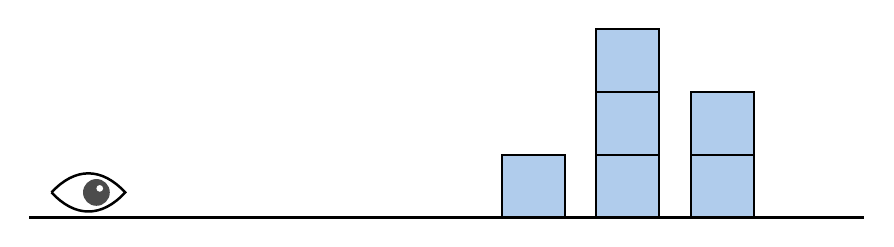
\begin{tikzpicture}
\draw[fill=cube, line width=0.7pt] (0.000,0.000) rectangle (0.800,0.800);
\draw[fill=cube, line width=0.7pt] (1.200,0.000) rectangle (2.000,0.800);
\draw[fill=cube, line width=0.7pt] (1.200,0.800) rectangle (2.000,1.600);
\draw[fill=cube, line width=0.7pt] (1.200,1.600) rectangle (2.000,2.400);
\draw[fill=cube, line width=0.7pt] (2.400,0.000) rectangle (3.200,0.800);
\draw[fill=cube, line width=0.7pt] (2.400,0.800) rectangle (3.200,1.600);
\draw[line width=1.2pt] (-6.000,0) -- (4.600,0);
\begin{scope}[shift={(-5.250,0.320)}, xscale=0.850, yscale=0.850]
\draw[line width=0.9pt, fill=white] (-0.55,0) .. controls (-0.2,0.38) and (0.2,0.38) .. (0.55,0) .. controls (0.2,-0.38) and (-0.2,-0.38) .. (-0.55,0);
\fill[black!70] (0.12,0) circle (0.2);
\fill[white] (0.17,0.06) circle (0.05);
\end{scope}
\end{tikzpicture}
\end{center}
\vspace{0.2cm}
\begin{minipage}{\linewidth}\RaggedRight
\prob{1}Make towers of 1, 2, and 3 cubes. Build each row in the picture, and write in each circle how many towers you see from that end.
\begin{center}
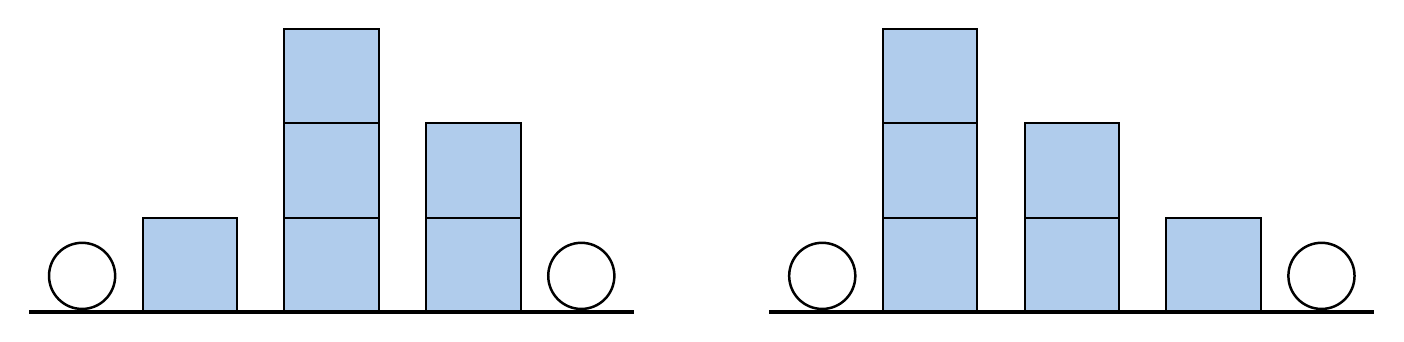
\begin{tikzpicture}
\begin{scope}[shift={(0.000,0.000)}]
\draw[fill=cube, line width=0.7pt] (0.000,0.000) rectangle (1.200,1.200);
\draw[fill=cube, line width=0.7pt] (1.800,0.000) rectangle (3.000,1.200);
\draw[fill=cube, line width=0.7pt] (1.800,1.200) rectangle (3.000,2.400);
\draw[fill=cube, line width=0.7pt] (1.800,2.400) rectangle (3.000,3.600);
\draw[fill=cube, line width=0.7pt] (3.600,0.000) rectangle (4.800,1.200);
\draw[fill=cube, line width=0.7pt] (3.600,1.200) rectangle (4.800,2.400);
\draw[line width=1.2pt] (-1.440,0) -- (6.240,0);
\draw[line width=0.9pt] (-0.770,0.460) circle (0.420);
\draw[line width=0.9pt] (5.570,0.460) circle (0.420);
\end{scope}
\begin{scope}[shift={(9.400,0.000)}]
\draw[fill=cube, line width=0.7pt] (0.000,0.000) rectangle (1.200,1.200);
\draw[fill=cube, line width=0.7pt] (0.000,1.200) rectangle (1.200,2.400);
\draw[fill=cube, line width=0.7pt] (0.000,2.400) rectangle (1.200,3.600);
\draw[fill=cube, line width=0.7pt] (1.800,0.000) rectangle (3.000,1.200);
\draw[fill=cube, line width=0.7pt] (1.800,1.200) rectangle (3.000,2.400);
\draw[fill=cube, line width=0.7pt] (3.600,0.000) rectangle (4.800,1.200);
\draw[line width=1.2pt] (-1.440,0) -- (6.240,0);
\draw[line width=0.9pt] (-0.770,0.460) circle (0.420);
\draw[line width=0.9pt] (5.570,0.460) circle (0.420);
\end{scope}
\end{tikzpicture}
\end{center}
\end{minipage}
\par\vspace{0.75cm}
\newpage
\begin{minipage}{\linewidth}\RaggedRight
\prob{2}Find every different way to stand your three towers in a row. Draw each way, and write how many towers you see from each end.
\vspace*{0.3cm}
\begin{center}
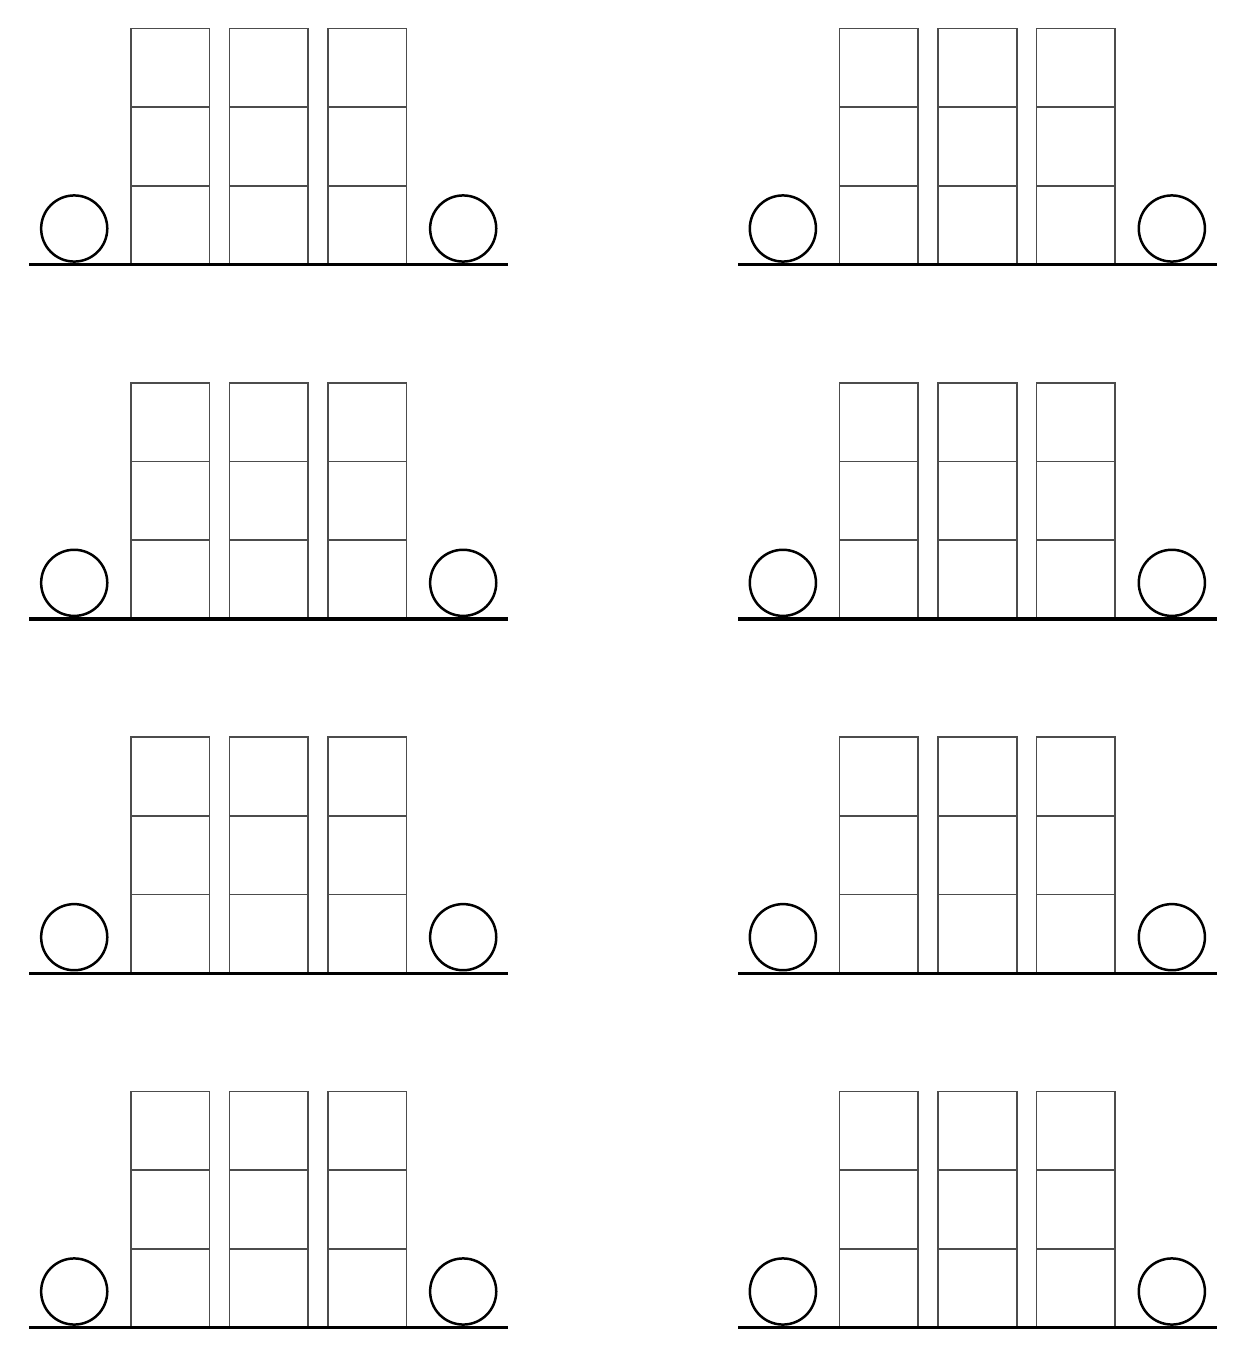
\begin{tikzpicture}
\begin{scope}[shift={(0.000,0.000)}]
\draw[line width=0.6pt, black!70] (0.000,0.000) rectangle (1.000,1.000);
\draw[line width=0.6pt, black!70] (0.000,1.000) rectangle (1.000,2.000);
\draw[line width=0.6pt, black!70] (0.000,2.000) rectangle (1.000,3.000);
\draw[line width=0.6pt, black!70] (1.250,0.000) rectangle (2.250,1.000);
\draw[line width=0.6pt, black!70] (1.250,1.000) rectangle (2.250,2.000);
\draw[line width=0.6pt, black!70] (1.250,2.000) rectangle (2.250,3.000);
\draw[line width=0.6pt, black!70] (2.500,0.000) rectangle (3.500,1.000);
\draw[line width=0.6pt, black!70] (2.500,1.000) rectangle (3.500,2.000);
\draw[line width=0.6pt, black!70] (2.500,2.000) rectangle (3.500,3.000);
\draw[line width=1.2pt] (-1.290,0) -- (4.790,0);
\draw[line width=0.9pt] (-0.720,0.460) circle (0.420);
\draw[line width=0.9pt] (4.220,0.460) circle (0.420);
\end{scope}
\begin{scope}[shift={(9.000,0.000)}]
\draw[line width=0.6pt, black!70] (0.000,0.000) rectangle (1.000,1.000);
\draw[line width=0.6pt, black!70] (0.000,1.000) rectangle (1.000,2.000);
\draw[line width=0.6pt, black!70] (0.000,2.000) rectangle (1.000,3.000);
\draw[line width=0.6pt, black!70] (1.250,0.000) rectangle (2.250,1.000);
\draw[line width=0.6pt, black!70] (1.250,1.000) rectangle (2.250,2.000);
\draw[line width=0.6pt, black!70] (1.250,2.000) rectangle (2.250,3.000);
\draw[line width=0.6pt, black!70] (2.500,0.000) rectangle (3.500,1.000);
\draw[line width=0.6pt, black!70] (2.500,1.000) rectangle (3.500,2.000);
\draw[line width=0.6pt, black!70] (2.500,2.000) rectangle (3.500,3.000);
\draw[line width=1.2pt] (-1.290,0) -- (4.790,0);
\draw[line width=0.9pt] (-0.720,0.460) circle (0.420);
\draw[line width=0.9pt] (4.220,0.460) circle (0.420);
\end{scope}
\begin{scope}[shift={(0.000,-4.500)}]
\draw[line width=0.6pt, black!70] (0.000,0.000) rectangle (1.000,1.000);
\draw[line width=0.6pt, black!70] (0.000,1.000) rectangle (1.000,2.000);
\draw[line width=0.6pt, black!70] (0.000,2.000) rectangle (1.000,3.000);
\draw[line width=0.6pt, black!70] (1.250,0.000) rectangle (2.250,1.000);
\draw[line width=0.6pt, black!70] (1.250,1.000) rectangle (2.250,2.000);
\draw[line width=0.6pt, black!70] (1.250,2.000) rectangle (2.250,3.000);
\draw[line width=0.6pt, black!70] (2.500,0.000) rectangle (3.500,1.000);
\draw[line width=0.6pt, black!70] (2.500,1.000) rectangle (3.500,2.000);
\draw[line width=0.6pt, black!70] (2.500,2.000) rectangle (3.500,3.000);
\draw[line width=1.2pt] (-1.290,0) -- (4.790,0);
\draw[line width=0.9pt] (-0.720,0.460) circle (0.420);
\draw[line width=0.9pt] (4.220,0.460) circle (0.420);
\end{scope}
\begin{scope}[shift={(9.000,-4.500)}]
\draw[line width=0.6pt, black!70] (0.000,0.000) rectangle (1.000,1.000);
\draw[line width=0.6pt, black!70] (0.000,1.000) rectangle (1.000,2.000);
\draw[line width=0.6pt, black!70] (0.000,2.000) rectangle (1.000,3.000);
\draw[line width=0.6pt, black!70] (1.250,0.000) rectangle (2.250,1.000);
\draw[line width=0.6pt, black!70] (1.250,1.000) rectangle (2.250,2.000);
\draw[line width=0.6pt, black!70] (1.250,2.000) rectangle (2.250,3.000);
\draw[line width=0.6pt, black!70] (2.500,0.000) rectangle (3.500,1.000);
\draw[line width=0.6pt, black!70] (2.500,1.000) rectangle (3.500,2.000);
\draw[line width=0.6pt, black!70] (2.500,2.000) rectangle (3.500,3.000);
\draw[line width=1.2pt] (-1.290,0) -- (4.790,0);
\draw[line width=0.9pt] (-0.720,0.460) circle (0.420);
\draw[line width=0.9pt] (4.220,0.460) circle (0.420);
\end{scope}
\begin{scope}[shift={(0.000,-9.000)}]
\draw[line width=0.6pt, black!70] (0.000,0.000) rectangle (1.000,1.000);
\draw[line width=0.6pt, black!70] (0.000,1.000) rectangle (1.000,2.000);
\draw[line width=0.6pt, black!70] (0.000,2.000) rectangle (1.000,3.000);
\draw[line width=0.6pt, black!70] (1.250,0.000) rectangle (2.250,1.000);
\draw[line width=0.6pt, black!70] (1.250,1.000) rectangle (2.250,2.000);
\draw[line width=0.6pt, black!70] (1.250,2.000) rectangle (2.250,3.000);
\draw[line width=0.6pt, black!70] (2.500,0.000) rectangle (3.500,1.000);
\draw[line width=0.6pt, black!70] (2.500,1.000) rectangle (3.500,2.000);
\draw[line width=0.6pt, black!70] (2.500,2.000) rectangle (3.500,3.000);
\draw[line width=1.2pt] (-1.290,0) -- (4.790,0);
\draw[line width=0.9pt] (-0.720,0.460) circle (0.420);
\draw[line width=0.9pt] (4.220,0.460) circle (0.420);
\end{scope}
\begin{scope}[shift={(9.000,-9.000)}]
\draw[line width=0.6pt, black!70] (0.000,0.000) rectangle (1.000,1.000);
\draw[line width=0.6pt, black!70] (0.000,1.000) rectangle (1.000,2.000);
\draw[line width=0.6pt, black!70] (0.000,2.000) rectangle (1.000,3.000);
\draw[line width=0.6pt, black!70] (1.250,0.000) rectangle (2.250,1.000);
\draw[line width=0.6pt, black!70] (1.250,1.000) rectangle (2.250,2.000);
\draw[line width=0.6pt, black!70] (1.250,2.000) rectangle (2.250,3.000);
\draw[line width=0.6pt, black!70] (2.500,0.000) rectangle (3.500,1.000);
\draw[line width=0.6pt, black!70] (2.500,1.000) rectangle (3.500,2.000);
\draw[line width=0.6pt, black!70] (2.500,2.000) rectangle (3.500,3.000);
\draw[line width=1.2pt] (-1.290,0) -- (4.790,0);
\draw[line width=0.9pt] (-0.720,0.460) circle (0.420);
\draw[line width=0.9pt] (4.220,0.460) circle (0.420);
\end{scope}
\begin{scope}[shift={(0.000,-13.500)}]
\draw[line width=0.6pt, black!70] (0.000,0.000) rectangle (1.000,1.000);
\draw[line width=0.6pt, black!70] (0.000,1.000) rectangle (1.000,2.000);
\draw[line width=0.6pt, black!70] (0.000,2.000) rectangle (1.000,3.000);
\draw[line width=0.6pt, black!70] (1.250,0.000) rectangle (2.250,1.000);
\draw[line width=0.6pt, black!70] (1.250,1.000) rectangle (2.250,2.000);
\draw[line width=0.6pt, black!70] (1.250,2.000) rectangle (2.250,3.000);
\draw[line width=0.6pt, black!70] (2.500,0.000) rectangle (3.500,1.000);
\draw[line width=0.6pt, black!70] (2.500,1.000) rectangle (3.500,2.000);
\draw[line width=0.6pt, black!70] (2.500,2.000) rectangle (3.500,3.000);
\draw[line width=1.2pt] (-1.290,0) -- (4.790,0);
\draw[line width=0.9pt] (-0.720,0.460) circle (0.420);
\draw[line width=0.9pt] (4.220,0.460) circle (0.420);
\end{scope}
\begin{scope}[shift={(9.000,-13.500)}]
\draw[line width=0.6pt, black!70] (0.000,0.000) rectangle (1.000,1.000);
\draw[line width=0.6pt, black!70] (0.000,1.000) rectangle (1.000,2.000);
\draw[line width=0.6pt, black!70] (0.000,2.000) rectangle (1.000,3.000);
\draw[line width=0.6pt, black!70] (1.250,0.000) rectangle (2.250,1.000);
\draw[line width=0.6pt, black!70] (1.250,1.000) rectangle (2.250,2.000);
\draw[line width=0.6pt, black!70] (1.250,2.000) rectangle (2.250,3.000);
\draw[line width=0.6pt, black!70] (2.500,0.000) rectangle (3.500,1.000);
\draw[line width=0.6pt, black!70] (2.500,1.000) rectangle (3.500,2.000);
\draw[line width=0.6pt, black!70] (2.500,2.000) rectangle (3.500,3.000);
\draw[line width=1.2pt] (-1.290,0) -- (4.790,0);
\draw[line width=0.9pt] (-0.720,0.460) circle (0.420);
\draw[line width=0.9pt] (4.220,0.460) circle (0.420);
\end{scope}
\end{tikzpicture}
\end{center}
\end{minipage}
\par\vspace{0.75cm}
\newpage
\begin{minipage}{\linewidth}\RaggedRight
\prob{3}Build a row of your three towers that shows the two numbers on each card, and draw it. If no row can, put an X on the card and tell why.
\vspace*{0.3cm}
\begin{center}
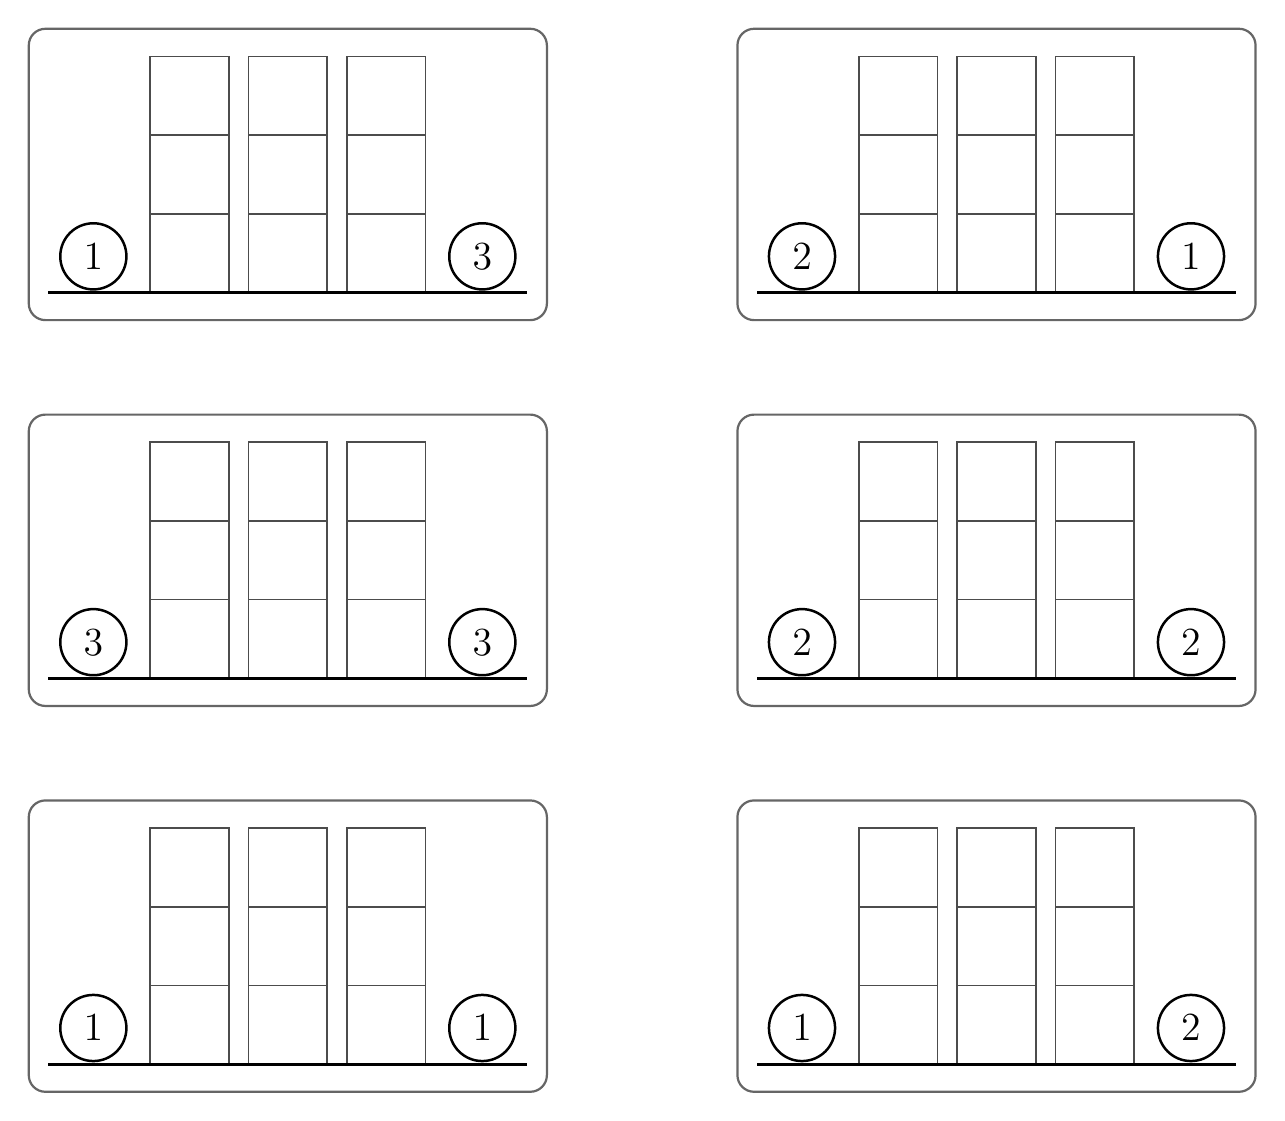
\begin{tikzpicture}
\begin{scope}[shift={(0.000,0.000)}]
\draw[line width=0.6pt, black!70] (0.000,0.000) rectangle (1.000,1.000);
\draw[line width=0.6pt, black!70] (0.000,1.000) rectangle (1.000,2.000);
\draw[line width=0.6pt, black!70] (0.000,2.000) rectangle (1.000,3.000);
\draw[line width=0.6pt, black!70] (1.250,0.000) rectangle (2.250,1.000);
\draw[line width=0.6pt, black!70] (1.250,1.000) rectangle (2.250,2.000);
\draw[line width=0.6pt, black!70] (1.250,2.000) rectangle (2.250,3.000);
\draw[line width=0.6pt, black!70] (2.500,0.000) rectangle (3.500,1.000);
\draw[line width=0.6pt, black!70] (2.500,1.000) rectangle (3.500,2.000);
\draw[line width=0.6pt, black!70] (2.500,2.000) rectangle (3.500,3.000);
\draw[line width=1.2pt] (-1.290,0) -- (4.790,0);
\draw[line width=0.9pt] (-0.720,0.460) circle (0.420);
\node at (-0.720,0.460) {\Large 1};
\draw[line width=0.9pt] (4.220,0.460) circle (0.420);
\node at (4.220,0.460) {\Large 3};
\draw[rounded corners=6pt, line width=0.8pt, black!60] (-1.540,-0.35) rectangle (5.040,3.350);
\end{scope}
\begin{scope}[shift={(9.000,0.000)}]
\draw[line width=0.6pt, black!70] (0.000,0.000) rectangle (1.000,1.000);
\draw[line width=0.6pt, black!70] (0.000,1.000) rectangle (1.000,2.000);
\draw[line width=0.6pt, black!70] (0.000,2.000) rectangle (1.000,3.000);
\draw[line width=0.6pt, black!70] (1.250,0.000) rectangle (2.250,1.000);
\draw[line width=0.6pt, black!70] (1.250,1.000) rectangle (2.250,2.000);
\draw[line width=0.6pt, black!70] (1.250,2.000) rectangle (2.250,3.000);
\draw[line width=0.6pt, black!70] (2.500,0.000) rectangle (3.500,1.000);
\draw[line width=0.6pt, black!70] (2.500,1.000) rectangle (3.500,2.000);
\draw[line width=0.6pt, black!70] (2.500,2.000) rectangle (3.500,3.000);
\draw[line width=1.2pt] (-1.290,0) -- (4.790,0);
\draw[line width=0.9pt] (-0.720,0.460) circle (0.420);
\node at (-0.720,0.460) {\Large 2};
\draw[line width=0.9pt] (4.220,0.460) circle (0.420);
\node at (4.220,0.460) {\Large 1};
\draw[rounded corners=6pt, line width=0.8pt, black!60] (-1.540,-0.35) rectangle (5.040,3.350);
\end{scope}
\begin{scope}[shift={(0.000,-4.900)}]
\draw[line width=0.6pt, black!70] (0.000,0.000) rectangle (1.000,1.000);
\draw[line width=0.6pt, black!70] (0.000,1.000) rectangle (1.000,2.000);
\draw[line width=0.6pt, black!70] (0.000,2.000) rectangle (1.000,3.000);
\draw[line width=0.6pt, black!70] (1.250,0.000) rectangle (2.250,1.000);
\draw[line width=0.6pt, black!70] (1.250,1.000) rectangle (2.250,2.000);
\draw[line width=0.6pt, black!70] (1.250,2.000) rectangle (2.250,3.000);
\draw[line width=0.6pt, black!70] (2.500,0.000) rectangle (3.500,1.000);
\draw[line width=0.6pt, black!70] (2.500,1.000) rectangle (3.500,2.000);
\draw[line width=0.6pt, black!70] (2.500,2.000) rectangle (3.500,3.000);
\draw[line width=1.2pt] (-1.290,0) -- (4.790,0);
\draw[line width=0.9pt] (-0.720,0.460) circle (0.420);
\node at (-0.720,0.460) {\Large 3};
\draw[line width=0.9pt] (4.220,0.460) circle (0.420);
\node at (4.220,0.460) {\Large 3};
\draw[rounded corners=6pt, line width=0.8pt, black!60] (-1.540,-0.35) rectangle (5.040,3.350);
\end{scope}
\begin{scope}[shift={(9.000,-4.900)}]
\draw[line width=0.6pt, black!70] (0.000,0.000) rectangle (1.000,1.000);
\draw[line width=0.6pt, black!70] (0.000,1.000) rectangle (1.000,2.000);
\draw[line width=0.6pt, black!70] (0.000,2.000) rectangle (1.000,3.000);
\draw[line width=0.6pt, black!70] (1.250,0.000) rectangle (2.250,1.000);
\draw[line width=0.6pt, black!70] (1.250,1.000) rectangle (2.250,2.000);
\draw[line width=0.6pt, black!70] (1.250,2.000) rectangle (2.250,3.000);
\draw[line width=0.6pt, black!70] (2.500,0.000) rectangle (3.500,1.000);
\draw[line width=0.6pt, black!70] (2.500,1.000) rectangle (3.500,2.000);
\draw[line width=0.6pt, black!70] (2.500,2.000) rectangle (3.500,3.000);
\draw[line width=1.2pt] (-1.290,0) -- (4.790,0);
\draw[line width=0.9pt] (-0.720,0.460) circle (0.420);
\node at (-0.720,0.460) {\Large 2};
\draw[line width=0.9pt] (4.220,0.460) circle (0.420);
\node at (4.220,0.460) {\Large 2};
\draw[rounded corners=6pt, line width=0.8pt, black!60] (-1.540,-0.35) rectangle (5.040,3.350);
\end{scope}
\begin{scope}[shift={(0.000,-9.800)}]
\draw[line width=0.6pt, black!70] (0.000,0.000) rectangle (1.000,1.000);
\draw[line width=0.6pt, black!70] (0.000,1.000) rectangle (1.000,2.000);
\draw[line width=0.6pt, black!70] (0.000,2.000) rectangle (1.000,3.000);
\draw[line width=0.6pt, black!70] (1.250,0.000) rectangle (2.250,1.000);
\draw[line width=0.6pt, black!70] (1.250,1.000) rectangle (2.250,2.000);
\draw[line width=0.6pt, black!70] (1.250,2.000) rectangle (2.250,3.000);
\draw[line width=0.6pt, black!70] (2.500,0.000) rectangle (3.500,1.000);
\draw[line width=0.6pt, black!70] (2.500,1.000) rectangle (3.500,2.000);
\draw[line width=0.6pt, black!70] (2.500,2.000) rectangle (3.500,3.000);
\draw[line width=1.2pt] (-1.290,0) -- (4.790,0);
\draw[line width=0.9pt] (-0.720,0.460) circle (0.420);
\node at (-0.720,0.460) {\Large 1};
\draw[line width=0.9pt] (4.220,0.460) circle (0.420);
\node at (4.220,0.460) {\Large 1};
\draw[rounded corners=6pt, line width=0.8pt, black!60] (-1.540,-0.35) rectangle (5.040,3.350);
\end{scope}
\begin{scope}[shift={(9.000,-9.800)}]
\draw[line width=0.6pt, black!70] (0.000,0.000) rectangle (1.000,1.000);
\draw[line width=0.6pt, black!70] (0.000,1.000) rectangle (1.000,2.000);
\draw[line width=0.6pt, black!70] (0.000,2.000) rectangle (1.000,3.000);
\draw[line width=0.6pt, black!70] (1.250,0.000) rectangle (2.250,1.000);
\draw[line width=0.6pt, black!70] (1.250,1.000) rectangle (2.250,2.000);
\draw[line width=0.6pt, black!70] (1.250,2.000) rectangle (2.250,3.000);
\draw[line width=0.6pt, black!70] (2.500,0.000) rectangle (3.500,1.000);
\draw[line width=0.6pt, black!70] (2.500,1.000) rectangle (3.500,2.000);
\draw[line width=0.6pt, black!70] (2.500,2.000) rectangle (3.500,3.000);
\draw[line width=1.2pt] (-1.290,0) -- (4.790,0);
\draw[line width=0.9pt] (-0.720,0.460) circle (0.420);
\node at (-0.720,0.460) {\Large 1};
\draw[line width=0.9pt] (4.220,0.460) circle (0.420);
\node at (4.220,0.460) {\Large 2};
\draw[rounded corners=6pt, line width=0.8pt, black!60] (-1.540,-0.35) rectangle (5.040,3.350);
\end{scope}
\end{tikzpicture}
\end{center}
\end{minipage}
\par\vspace{0.75cm}
\newpage
\begin{minipage}{\linewidth}\RaggedRight
\prob{4}One partner hides a row of three towers behind a folder and says how many towers you can see from each end. The other builds a row that shows those numbers and draws it, and then you swap.
\begin{center}
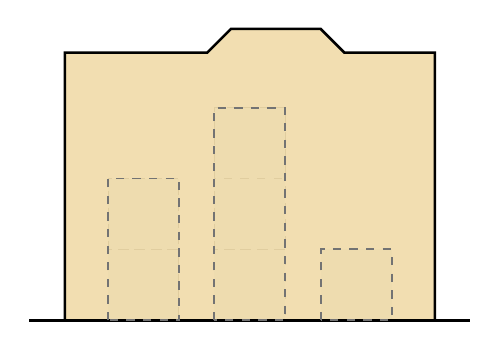
\begin{tikzpicture}
\draw[dashed, black!55, fill=cube!35] (0.000,0.000) rectangle (0.900,0.900);
\draw[dashed, black!55, fill=cube!35] (0.000,0.900) rectangle (0.900,1.800);
\draw[dashed, black!55, fill=cube!35] (1.350,0.000) rectangle (2.250,0.900);
\draw[dashed, black!55, fill=cube!35] (1.350,0.900) rectangle (2.250,1.800);
\draw[dashed, black!55, fill=cube!35] (1.350,1.800) rectangle (2.250,2.700);
\draw[dashed, black!55, fill=cube!35] (2.700,0.000) rectangle (3.600,0.900);
\draw[line width=1.2pt] (-1.000,0) -- (4.600,0);
\draw[line width=0.9pt, fill=folder, fill opacity=0.88] (-0.550,0) -- (-0.550,3.400) -- (1.260,3.400) -- (1.560,3.700) -- (2.700,3.700) -- (3.000,3.400) -- (4.150,3.400) -- (4.150,0) -- cycle;
\draw[dashed, black!55, line width=0.7pt] (0.000,0) rectangle (0.900,1.800);
\draw[dashed, black!55, line width=0.7pt] (1.350,0) rectangle (2.250,2.700);
\draw[dashed, black!55, line width=0.7pt] (2.700,0) rectangle (3.600,0.900);
\end{tikzpicture}
\end{center}
\vspace*{0.3cm}
\begin{center}
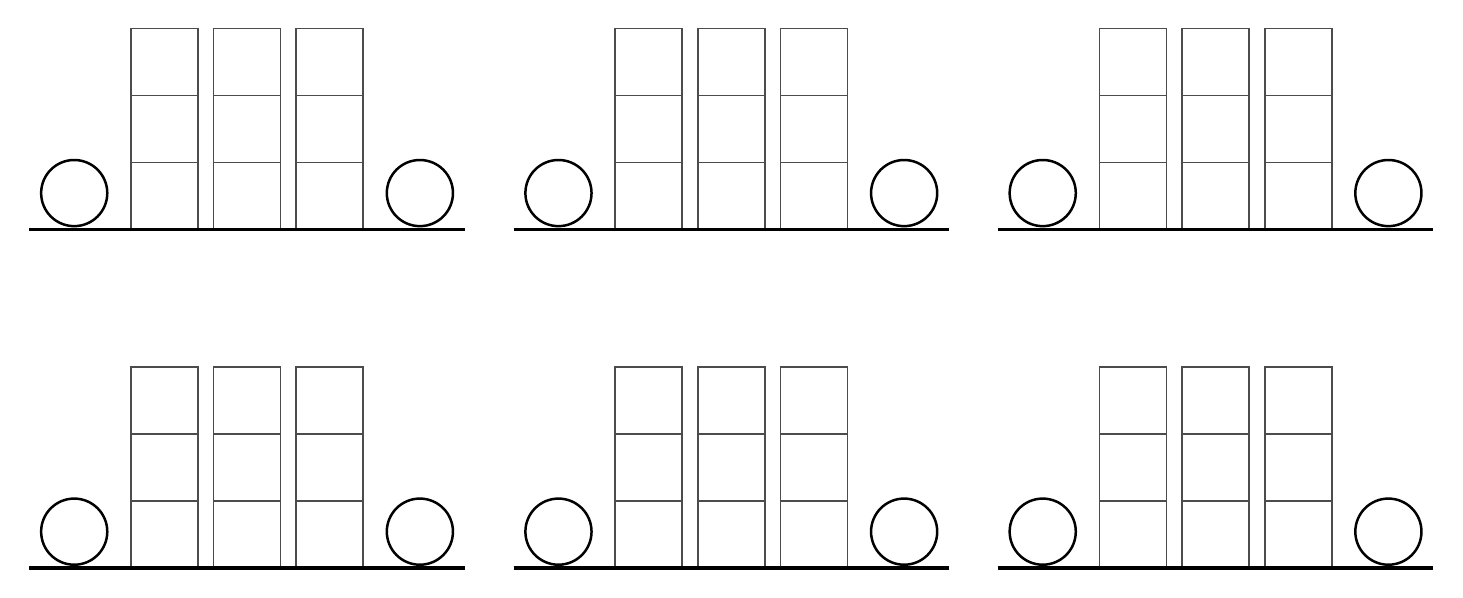
\begin{tikzpicture}
\begin{scope}[shift={(0.000,0.000)}]
\draw[line width=0.6pt, black!70] (0.000,0.000) rectangle (0.850,0.850);
\draw[line width=0.6pt, black!70] (0.000,0.850) rectangle (0.850,1.700);
\draw[line width=0.6pt, black!70] (0.000,1.700) rectangle (0.850,2.550);
\draw[line width=0.6pt, black!70] (1.050,0.000) rectangle (1.900,0.850);
\draw[line width=0.6pt, black!70] (1.050,0.850) rectangle (1.900,1.700);
\draw[line width=0.6pt, black!70] (1.050,1.700) rectangle (1.900,2.550);
\draw[line width=0.6pt, black!70] (2.100,0.000) rectangle (2.950,0.850);
\draw[line width=0.6pt, black!70] (2.100,0.850) rectangle (2.950,1.700);
\draw[line width=0.6pt, black!70] (2.100,1.700) rectangle (2.950,2.550);
\draw[line width=1.2pt] (-1.290,0) -- (4.240,0);
\draw[line width=0.9pt] (-0.720,0.460) circle (0.420);
\draw[line width=0.9pt] (3.670,0.460) circle (0.420);
\end{scope}
\begin{scope}[shift={(6.150,0.000)}]
\draw[line width=0.6pt, black!70] (0.000,0.000) rectangle (0.850,0.850);
\draw[line width=0.6pt, black!70] (0.000,0.850) rectangle (0.850,1.700);
\draw[line width=0.6pt, black!70] (0.000,1.700) rectangle (0.850,2.550);
\draw[line width=0.6pt, black!70] (1.050,0.000) rectangle (1.900,0.850);
\draw[line width=0.6pt, black!70] (1.050,0.850) rectangle (1.900,1.700);
\draw[line width=0.6pt, black!70] (1.050,1.700) rectangle (1.900,2.550);
\draw[line width=0.6pt, black!70] (2.100,0.000) rectangle (2.950,0.850);
\draw[line width=0.6pt, black!70] (2.100,0.850) rectangle (2.950,1.700);
\draw[line width=0.6pt, black!70] (2.100,1.700) rectangle (2.950,2.550);
\draw[line width=1.2pt] (-1.290,0) -- (4.240,0);
\draw[line width=0.9pt] (-0.720,0.460) circle (0.420);
\draw[line width=0.9pt] (3.670,0.460) circle (0.420);
\end{scope}
\begin{scope}[shift={(12.300,0.000)}]
\draw[line width=0.6pt, black!70] (0.000,0.000) rectangle (0.850,0.850);
\draw[line width=0.6pt, black!70] (0.000,0.850) rectangle (0.850,1.700);
\draw[line width=0.6pt, black!70] (0.000,1.700) rectangle (0.850,2.550);
\draw[line width=0.6pt, black!70] (1.050,0.000) rectangle (1.900,0.850);
\draw[line width=0.6pt, black!70] (1.050,0.850) rectangle (1.900,1.700);
\draw[line width=0.6pt, black!70] (1.050,1.700) rectangle (1.900,2.550);
\draw[line width=0.6pt, black!70] (2.100,0.000) rectangle (2.950,0.850);
\draw[line width=0.6pt, black!70] (2.100,0.850) rectangle (2.950,1.700);
\draw[line width=0.6pt, black!70] (2.100,1.700) rectangle (2.950,2.550);
\draw[line width=1.2pt] (-1.290,0) -- (4.240,0);
\draw[line width=0.9pt] (-0.720,0.460) circle (0.420);
\draw[line width=0.9pt] (3.670,0.460) circle (0.420);
\end{scope}
\begin{scope}[shift={(0.000,-4.300)}]
\draw[line width=0.6pt, black!70] (0.000,0.000) rectangle (0.850,0.850);
\draw[line width=0.6pt, black!70] (0.000,0.850) rectangle (0.850,1.700);
\draw[line width=0.6pt, black!70] (0.000,1.700) rectangle (0.850,2.550);
\draw[line width=0.6pt, black!70] (1.050,0.000) rectangle (1.900,0.850);
\draw[line width=0.6pt, black!70] (1.050,0.850) rectangle (1.900,1.700);
\draw[line width=0.6pt, black!70] (1.050,1.700) rectangle (1.900,2.550);
\draw[line width=0.6pt, black!70] (2.100,0.000) rectangle (2.950,0.850);
\draw[line width=0.6pt, black!70] (2.100,0.850) rectangle (2.950,1.700);
\draw[line width=0.6pt, black!70] (2.100,1.700) rectangle (2.950,2.550);
\draw[line width=1.2pt] (-1.290,0) -- (4.240,0);
\draw[line width=0.9pt] (-0.720,0.460) circle (0.420);
\draw[line width=0.9pt] (3.670,0.460) circle (0.420);
\end{scope}
\begin{scope}[shift={(6.150,-4.300)}]
\draw[line width=0.6pt, black!70] (0.000,0.000) rectangle (0.850,0.850);
\draw[line width=0.6pt, black!70] (0.000,0.850) rectangle (0.850,1.700);
\draw[line width=0.6pt, black!70] (0.000,1.700) rectangle (0.850,2.550);
\draw[line width=0.6pt, black!70] (1.050,0.000) rectangle (1.900,0.850);
\draw[line width=0.6pt, black!70] (1.050,0.850) rectangle (1.900,1.700);
\draw[line width=0.6pt, black!70] (1.050,1.700) rectangle (1.900,2.550);
\draw[line width=0.6pt, black!70] (2.100,0.000) rectangle (2.950,0.850);
\draw[line width=0.6pt, black!70] (2.100,0.850) rectangle (2.950,1.700);
\draw[line width=0.6pt, black!70] (2.100,1.700) rectangle (2.950,2.550);
\draw[line width=1.2pt] (-1.290,0) -- (4.240,0);
\draw[line width=0.9pt] (-0.720,0.460) circle (0.420);
\draw[line width=0.9pt] (3.670,0.460) circle (0.420);
\end{scope}
\begin{scope}[shift={(12.300,-4.300)}]
\draw[line width=0.6pt, black!70] (0.000,0.000) rectangle (0.850,0.850);
\draw[line width=0.6pt, black!70] (0.000,0.850) rectangle (0.850,1.700);
\draw[line width=0.6pt, black!70] (0.000,1.700) rectangle (0.850,2.550);
\draw[line width=0.6pt, black!70] (1.050,0.000) rectangle (1.900,0.850);
\draw[line width=0.6pt, black!70] (1.050,0.850) rectangle (1.900,1.700);
\draw[line width=0.6pt, black!70] (1.050,1.700) rectangle (1.900,2.550);
\draw[line width=0.6pt, black!70] (2.100,0.000) rectangle (2.950,0.850);
\draw[line width=0.6pt, black!70] (2.100,0.850) rectangle (2.950,1.700);
\draw[line width=0.6pt, black!70] (2.100,1.700) rectangle (2.950,2.550);
\draw[line width=1.2pt] (-1.290,0) -- (4.240,0);
\draw[line width=0.9pt] (-0.720,0.460) circle (0.420);
\draw[line width=0.9pt] (3.670,0.460) circle (0.420);
\end{scope}
\end{tikzpicture}
\end{center}
\end{minipage}
\par\vspace{0.75cm}
\newpage
\begin{minipage}{\linewidth}\RaggedRight
\prob{5}Put your cubes together with your partner's and make towers of 1, 2, 3, and 4 cubes. Find and draw every row of these four towers where you see just 1 tower from the left end. How do you know you have them all?
\vspace*{0.3cm}
\begin{center}
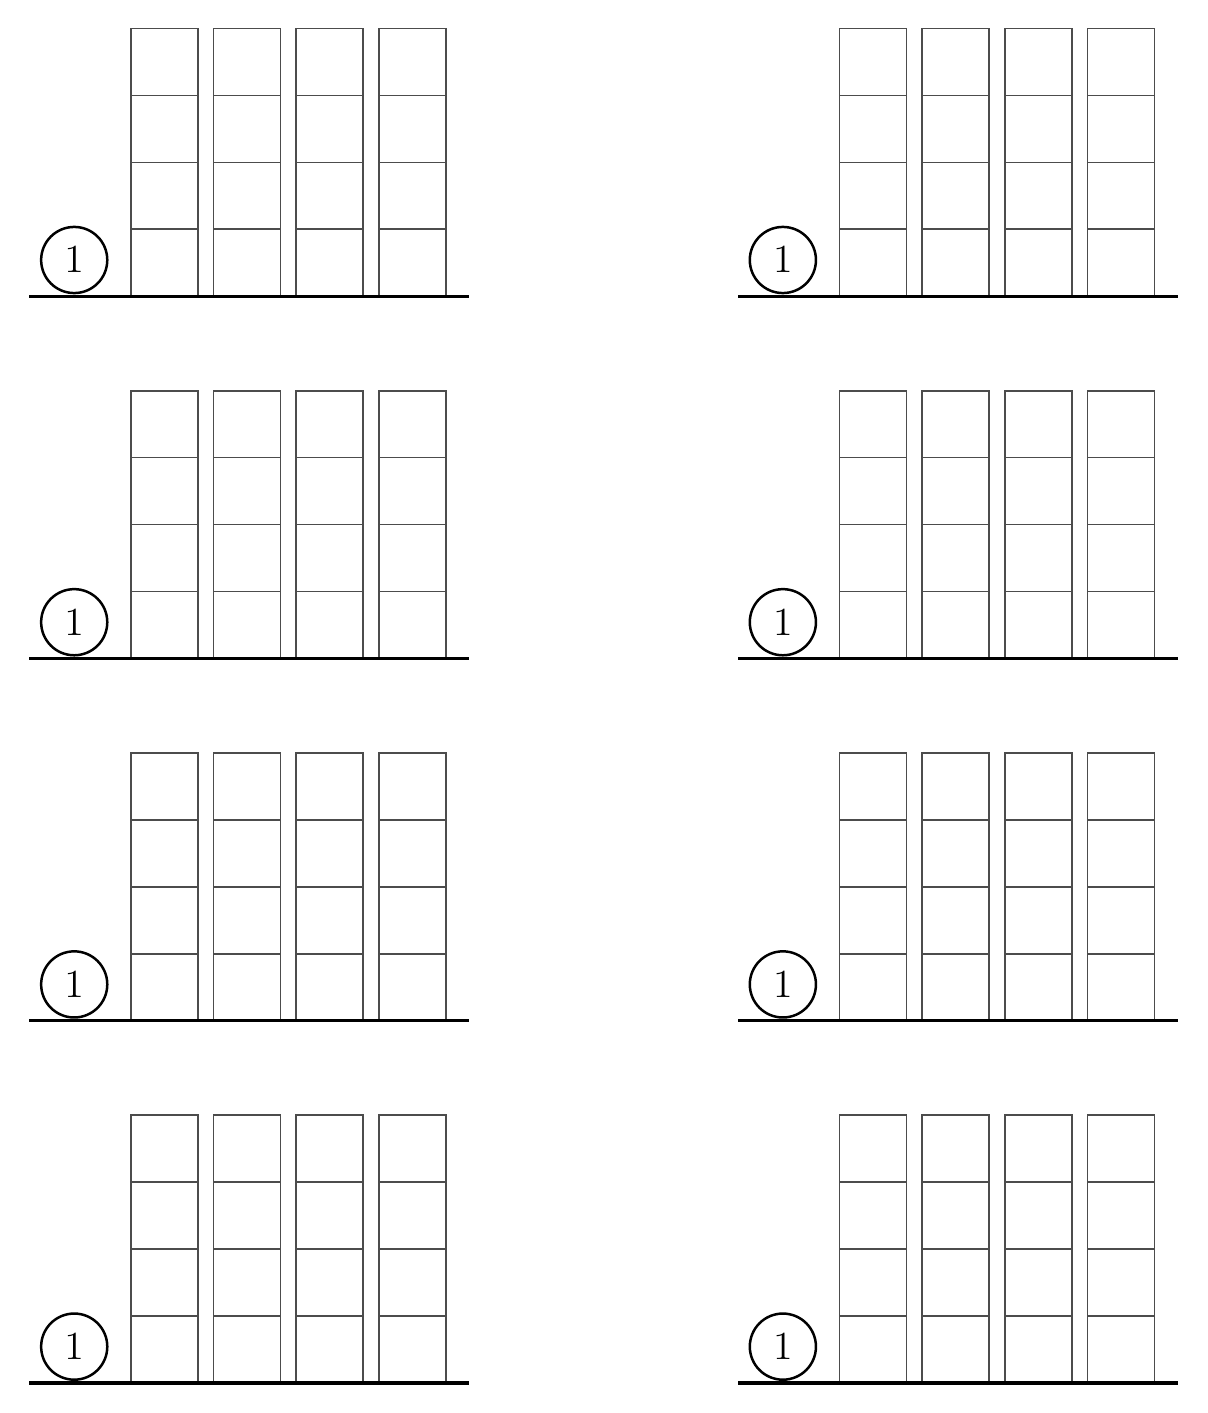
\begin{tikzpicture}
\begin{scope}[shift={(0.000,0.000)}]
\draw[line width=0.6pt, black!70] (0.000,0.000) rectangle (0.850,0.850);
\draw[line width=0.6pt, black!70] (0.000,0.850) rectangle (0.850,1.700);
\draw[line width=0.6pt, black!70] (0.000,1.700) rectangle (0.850,2.550);
\draw[line width=0.6pt, black!70] (0.000,2.550) rectangle (0.850,3.400);
\draw[line width=0.6pt, black!70] (1.050,0.000) rectangle (1.900,0.850);
\draw[line width=0.6pt, black!70] (1.050,0.850) rectangle (1.900,1.700);
\draw[line width=0.6pt, black!70] (1.050,1.700) rectangle (1.900,2.550);
\draw[line width=0.6pt, black!70] (1.050,2.550) rectangle (1.900,3.400);
\draw[line width=0.6pt, black!70] (2.100,0.000) rectangle (2.950,0.850);
\draw[line width=0.6pt, black!70] (2.100,0.850) rectangle (2.950,1.700);
\draw[line width=0.6pt, black!70] (2.100,1.700) rectangle (2.950,2.550);
\draw[line width=0.6pt, black!70] (2.100,2.550) rectangle (2.950,3.400);
\draw[line width=0.6pt, black!70] (3.150,0.000) rectangle (4.000,0.850);
\draw[line width=0.6pt, black!70] (3.150,0.850) rectangle (4.000,1.700);
\draw[line width=0.6pt, black!70] (3.150,1.700) rectangle (4.000,2.550);
\draw[line width=0.6pt, black!70] (3.150,2.550) rectangle (4.000,3.400);
\draw[line width=1.2pt] (-1.290,0) -- (4.300,0);
\draw[line width=0.9pt] (-0.720,0.460) circle (0.420);
\node at (-0.720,0.460) {\Large 1};
\end{scope}
\begin{scope}[shift={(9.000,0.000)}]
\draw[line width=0.6pt, black!70] (0.000,0.000) rectangle (0.850,0.850);
\draw[line width=0.6pt, black!70] (0.000,0.850) rectangle (0.850,1.700);
\draw[line width=0.6pt, black!70] (0.000,1.700) rectangle (0.850,2.550);
\draw[line width=0.6pt, black!70] (0.000,2.550) rectangle (0.850,3.400);
\draw[line width=0.6pt, black!70] (1.050,0.000) rectangle (1.900,0.850);
\draw[line width=0.6pt, black!70] (1.050,0.850) rectangle (1.900,1.700);
\draw[line width=0.6pt, black!70] (1.050,1.700) rectangle (1.900,2.550);
\draw[line width=0.6pt, black!70] (1.050,2.550) rectangle (1.900,3.400);
\draw[line width=0.6pt, black!70] (2.100,0.000) rectangle (2.950,0.850);
\draw[line width=0.6pt, black!70] (2.100,0.850) rectangle (2.950,1.700);
\draw[line width=0.6pt, black!70] (2.100,1.700) rectangle (2.950,2.550);
\draw[line width=0.6pt, black!70] (2.100,2.550) rectangle (2.950,3.400);
\draw[line width=0.6pt, black!70] (3.150,0.000) rectangle (4.000,0.850);
\draw[line width=0.6pt, black!70] (3.150,0.850) rectangle (4.000,1.700);
\draw[line width=0.6pt, black!70] (3.150,1.700) rectangle (4.000,2.550);
\draw[line width=0.6pt, black!70] (3.150,2.550) rectangle (4.000,3.400);
\draw[line width=1.2pt] (-1.290,0) -- (4.300,0);
\draw[line width=0.9pt] (-0.720,0.460) circle (0.420);
\node at (-0.720,0.460) {\Large 1};
\end{scope}
\begin{scope}[shift={(0.000,-4.600)}]
\draw[line width=0.6pt, black!70] (0.000,0.000) rectangle (0.850,0.850);
\draw[line width=0.6pt, black!70] (0.000,0.850) rectangle (0.850,1.700);
\draw[line width=0.6pt, black!70] (0.000,1.700) rectangle (0.850,2.550);
\draw[line width=0.6pt, black!70] (0.000,2.550) rectangle (0.850,3.400);
\draw[line width=0.6pt, black!70] (1.050,0.000) rectangle (1.900,0.850);
\draw[line width=0.6pt, black!70] (1.050,0.850) rectangle (1.900,1.700);
\draw[line width=0.6pt, black!70] (1.050,1.700) rectangle (1.900,2.550);
\draw[line width=0.6pt, black!70] (1.050,2.550) rectangle (1.900,3.400);
\draw[line width=0.6pt, black!70] (2.100,0.000) rectangle (2.950,0.850);
\draw[line width=0.6pt, black!70] (2.100,0.850) rectangle (2.950,1.700);
\draw[line width=0.6pt, black!70] (2.100,1.700) rectangle (2.950,2.550);
\draw[line width=0.6pt, black!70] (2.100,2.550) rectangle (2.950,3.400);
\draw[line width=0.6pt, black!70] (3.150,0.000) rectangle (4.000,0.850);
\draw[line width=0.6pt, black!70] (3.150,0.850) rectangle (4.000,1.700);
\draw[line width=0.6pt, black!70] (3.150,1.700) rectangle (4.000,2.550);
\draw[line width=0.6pt, black!70] (3.150,2.550) rectangle (4.000,3.400);
\draw[line width=1.2pt] (-1.290,0) -- (4.300,0);
\draw[line width=0.9pt] (-0.720,0.460) circle (0.420);
\node at (-0.720,0.460) {\Large 1};
\end{scope}
\begin{scope}[shift={(9.000,-4.600)}]
\draw[line width=0.6pt, black!70] (0.000,0.000) rectangle (0.850,0.850);
\draw[line width=0.6pt, black!70] (0.000,0.850) rectangle (0.850,1.700);
\draw[line width=0.6pt, black!70] (0.000,1.700) rectangle (0.850,2.550);
\draw[line width=0.6pt, black!70] (0.000,2.550) rectangle (0.850,3.400);
\draw[line width=0.6pt, black!70] (1.050,0.000) rectangle (1.900,0.850);
\draw[line width=0.6pt, black!70] (1.050,0.850) rectangle (1.900,1.700);
\draw[line width=0.6pt, black!70] (1.050,1.700) rectangle (1.900,2.550);
\draw[line width=0.6pt, black!70] (1.050,2.550) rectangle (1.900,3.400);
\draw[line width=0.6pt, black!70] (2.100,0.000) rectangle (2.950,0.850);
\draw[line width=0.6pt, black!70] (2.100,0.850) rectangle (2.950,1.700);
\draw[line width=0.6pt, black!70] (2.100,1.700) rectangle (2.950,2.550);
\draw[line width=0.6pt, black!70] (2.100,2.550) rectangle (2.950,3.400);
\draw[line width=0.6pt, black!70] (3.150,0.000) rectangle (4.000,0.850);
\draw[line width=0.6pt, black!70] (3.150,0.850) rectangle (4.000,1.700);
\draw[line width=0.6pt, black!70] (3.150,1.700) rectangle (4.000,2.550);
\draw[line width=0.6pt, black!70] (3.150,2.550) rectangle (4.000,3.400);
\draw[line width=1.2pt] (-1.290,0) -- (4.300,0);
\draw[line width=0.9pt] (-0.720,0.460) circle (0.420);
\node at (-0.720,0.460) {\Large 1};
\end{scope}
\begin{scope}[shift={(0.000,-9.200)}]
\draw[line width=0.6pt, black!70] (0.000,0.000) rectangle (0.850,0.850);
\draw[line width=0.6pt, black!70] (0.000,0.850) rectangle (0.850,1.700);
\draw[line width=0.6pt, black!70] (0.000,1.700) rectangle (0.850,2.550);
\draw[line width=0.6pt, black!70] (0.000,2.550) rectangle (0.850,3.400);
\draw[line width=0.6pt, black!70] (1.050,0.000) rectangle (1.900,0.850);
\draw[line width=0.6pt, black!70] (1.050,0.850) rectangle (1.900,1.700);
\draw[line width=0.6pt, black!70] (1.050,1.700) rectangle (1.900,2.550);
\draw[line width=0.6pt, black!70] (1.050,2.550) rectangle (1.900,3.400);
\draw[line width=0.6pt, black!70] (2.100,0.000) rectangle (2.950,0.850);
\draw[line width=0.6pt, black!70] (2.100,0.850) rectangle (2.950,1.700);
\draw[line width=0.6pt, black!70] (2.100,1.700) rectangle (2.950,2.550);
\draw[line width=0.6pt, black!70] (2.100,2.550) rectangle (2.950,3.400);
\draw[line width=0.6pt, black!70] (3.150,0.000) rectangle (4.000,0.850);
\draw[line width=0.6pt, black!70] (3.150,0.850) rectangle (4.000,1.700);
\draw[line width=0.6pt, black!70] (3.150,1.700) rectangle (4.000,2.550);
\draw[line width=0.6pt, black!70] (3.150,2.550) rectangle (4.000,3.400);
\draw[line width=1.2pt] (-1.290,0) -- (4.300,0);
\draw[line width=0.9pt] (-0.720,0.460) circle (0.420);
\node at (-0.720,0.460) {\Large 1};
\end{scope}
\begin{scope}[shift={(9.000,-9.200)}]
\draw[line width=0.6pt, black!70] (0.000,0.000) rectangle (0.850,0.850);
\draw[line width=0.6pt, black!70] (0.000,0.850) rectangle (0.850,1.700);
\draw[line width=0.6pt, black!70] (0.000,1.700) rectangle (0.850,2.550);
\draw[line width=0.6pt, black!70] (0.000,2.550) rectangle (0.850,3.400);
\draw[line width=0.6pt, black!70] (1.050,0.000) rectangle (1.900,0.850);
\draw[line width=0.6pt, black!70] (1.050,0.850) rectangle (1.900,1.700);
\draw[line width=0.6pt, black!70] (1.050,1.700) rectangle (1.900,2.550);
\draw[line width=0.6pt, black!70] (1.050,2.550) rectangle (1.900,3.400);
\draw[line width=0.6pt, black!70] (2.100,0.000) rectangle (2.950,0.850);
\draw[line width=0.6pt, black!70] (2.100,0.850) rectangle (2.950,1.700);
\draw[line width=0.6pt, black!70] (2.100,1.700) rectangle (2.950,2.550);
\draw[line width=0.6pt, black!70] (2.100,2.550) rectangle (2.950,3.400);
\draw[line width=0.6pt, black!70] (3.150,0.000) rectangle (4.000,0.850);
\draw[line width=0.6pt, black!70] (3.150,0.850) rectangle (4.000,1.700);
\draw[line width=0.6pt, black!70] (3.150,1.700) rectangle (4.000,2.550);
\draw[line width=0.6pt, black!70] (3.150,2.550) rectangle (4.000,3.400);
\draw[line width=1.2pt] (-1.290,0) -- (4.300,0);
\draw[line width=0.9pt] (-0.720,0.460) circle (0.420);
\node at (-0.720,0.460) {\Large 1};
\end{scope}
\begin{scope}[shift={(0.000,-13.800)}]
\draw[line width=0.6pt, black!70] (0.000,0.000) rectangle (0.850,0.850);
\draw[line width=0.6pt, black!70] (0.000,0.850) rectangle (0.850,1.700);
\draw[line width=0.6pt, black!70] (0.000,1.700) rectangle (0.850,2.550);
\draw[line width=0.6pt, black!70] (0.000,2.550) rectangle (0.850,3.400);
\draw[line width=0.6pt, black!70] (1.050,0.000) rectangle (1.900,0.850);
\draw[line width=0.6pt, black!70] (1.050,0.850) rectangle (1.900,1.700);
\draw[line width=0.6pt, black!70] (1.050,1.700) rectangle (1.900,2.550);
\draw[line width=0.6pt, black!70] (1.050,2.550) rectangle (1.900,3.400);
\draw[line width=0.6pt, black!70] (2.100,0.000) rectangle (2.950,0.850);
\draw[line width=0.6pt, black!70] (2.100,0.850) rectangle (2.950,1.700);
\draw[line width=0.6pt, black!70] (2.100,1.700) rectangle (2.950,2.550);
\draw[line width=0.6pt, black!70] (2.100,2.550) rectangle (2.950,3.400);
\draw[line width=0.6pt, black!70] (3.150,0.000) rectangle (4.000,0.850);
\draw[line width=0.6pt, black!70] (3.150,0.850) rectangle (4.000,1.700);
\draw[line width=0.6pt, black!70] (3.150,1.700) rectangle (4.000,2.550);
\draw[line width=0.6pt, black!70] (3.150,2.550) rectangle (4.000,3.400);
\draw[line width=1.2pt] (-1.290,0) -- (4.300,0);
\draw[line width=0.9pt] (-0.720,0.460) circle (0.420);
\node at (-0.720,0.460) {\Large 1};
\end{scope}
\begin{scope}[shift={(9.000,-13.800)}]
\draw[line width=0.6pt, black!70] (0.000,0.000) rectangle (0.850,0.850);
\draw[line width=0.6pt, black!70] (0.000,0.850) rectangle (0.850,1.700);
\draw[line width=0.6pt, black!70] (0.000,1.700) rectangle (0.850,2.550);
\draw[line width=0.6pt, black!70] (0.000,2.550) rectangle (0.850,3.400);
\draw[line width=0.6pt, black!70] (1.050,0.000) rectangle (1.900,0.850);
\draw[line width=0.6pt, black!70] (1.050,0.850) rectangle (1.900,1.700);
\draw[line width=0.6pt, black!70] (1.050,1.700) rectangle (1.900,2.550);
\draw[line width=0.6pt, black!70] (1.050,2.550) rectangle (1.900,3.400);
\draw[line width=0.6pt, black!70] (2.100,0.000) rectangle (2.950,0.850);
\draw[line width=0.6pt, black!70] (2.100,0.850) rectangle (2.950,1.700);
\draw[line width=0.6pt, black!70] (2.100,1.700) rectangle (2.950,2.550);
\draw[line width=0.6pt, black!70] (2.100,2.550) rectangle (2.950,3.400);
\draw[line width=0.6pt, black!70] (3.150,0.000) rectangle (4.000,0.850);
\draw[line width=0.6pt, black!70] (3.150,0.850) rectangle (4.000,1.700);
\draw[line width=0.6pt, black!70] (3.150,1.700) rectangle (4.000,2.550);
\draw[line width=0.6pt, black!70] (3.150,2.550) rectangle (4.000,3.400);
\draw[line width=1.2pt] (-1.290,0) -- (4.300,0);
\draw[line width=0.9pt] (-0.720,0.460) circle (0.420);
\node at (-0.720,0.460) {\Large 1};
\end{scope}
\end{tikzpicture}
\end{center}
\end{minipage}
\par\vspace{0.75cm}
\newpage
\begin{minipage}{\linewidth}\RaggedRight
\prob{6}Find and draw every row of your four towers where you see 2 towers from each end.
\vspace*{0.3cm}
\begin{center}
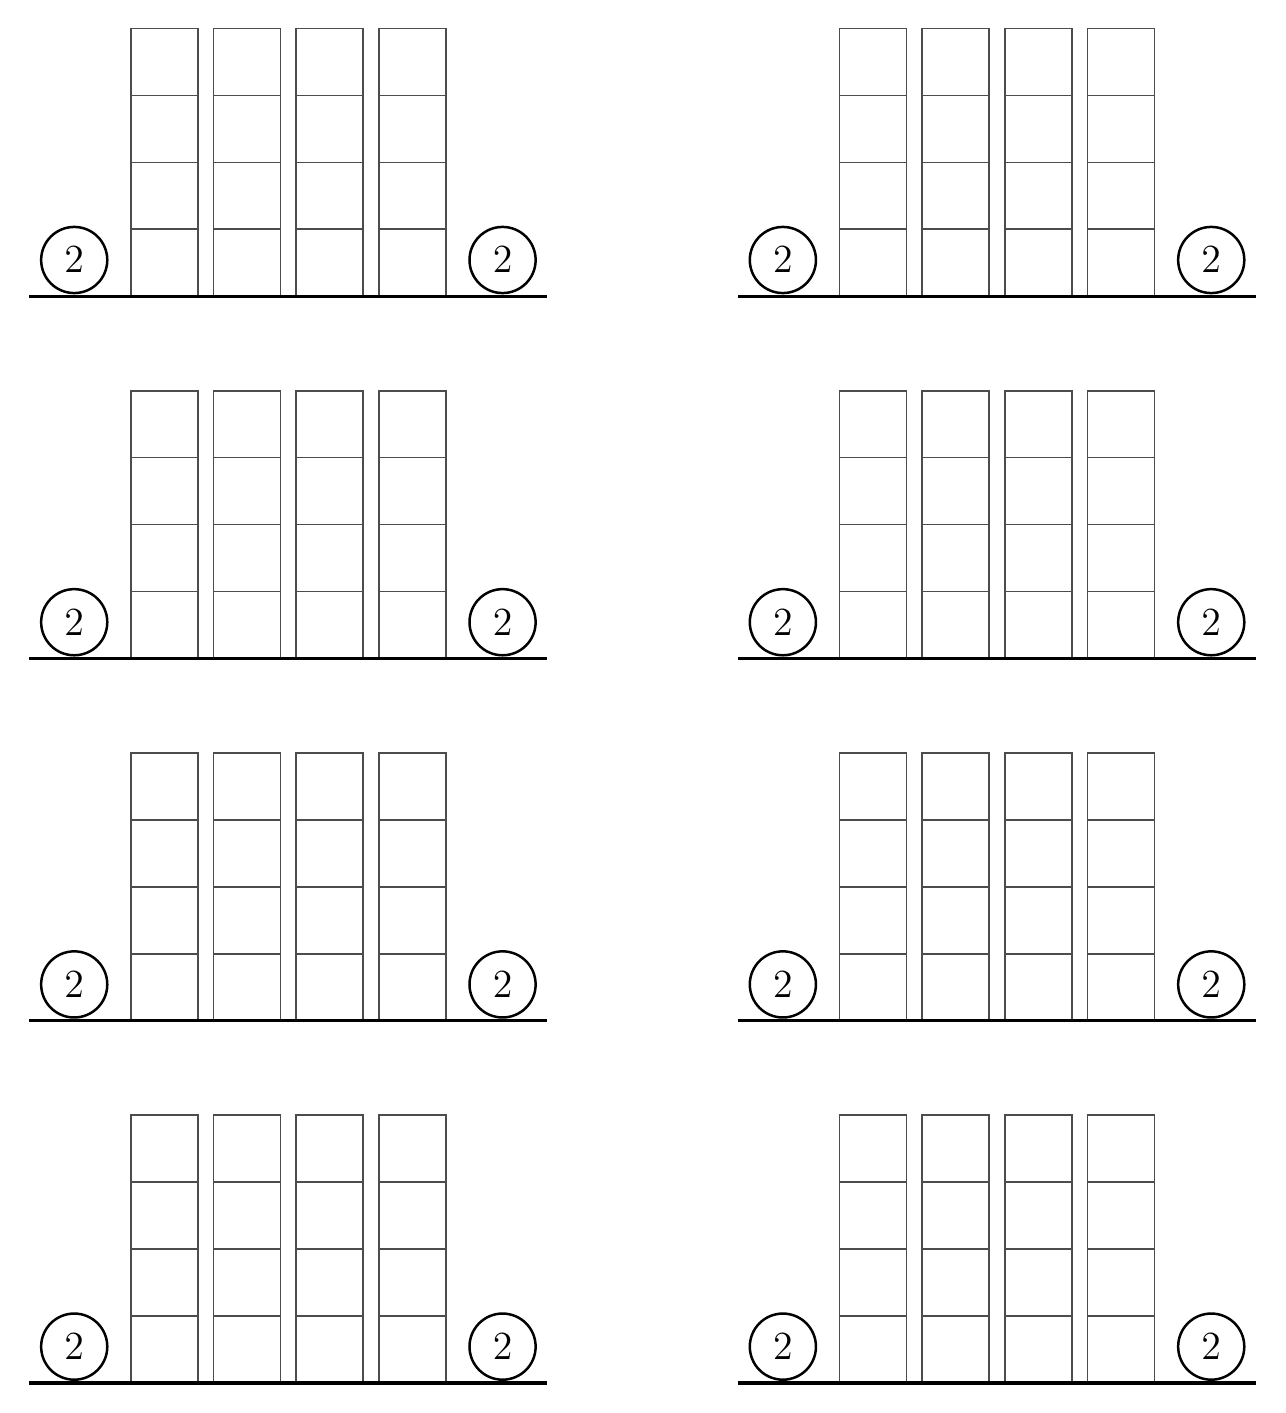
\begin{tikzpicture}
\begin{scope}[shift={(0.000,0.000)}]
\draw[line width=0.6pt, black!70] (0.000,0.000) rectangle (0.850,0.850);
\draw[line width=0.6pt, black!70] (0.000,0.850) rectangle (0.850,1.700);
\draw[line width=0.6pt, black!70] (0.000,1.700) rectangle (0.850,2.550);
\draw[line width=0.6pt, black!70] (0.000,2.550) rectangle (0.850,3.400);
\draw[line width=0.6pt, black!70] (1.050,0.000) rectangle (1.900,0.850);
\draw[line width=0.6pt, black!70] (1.050,0.850) rectangle (1.900,1.700);
\draw[line width=0.6pt, black!70] (1.050,1.700) rectangle (1.900,2.550);
\draw[line width=0.6pt, black!70] (1.050,2.550) rectangle (1.900,3.400);
\draw[line width=0.6pt, black!70] (2.100,0.000) rectangle (2.950,0.850);
\draw[line width=0.6pt, black!70] (2.100,0.850) rectangle (2.950,1.700);
\draw[line width=0.6pt, black!70] (2.100,1.700) rectangle (2.950,2.550);
\draw[line width=0.6pt, black!70] (2.100,2.550) rectangle (2.950,3.400);
\draw[line width=0.6pt, black!70] (3.150,0.000) rectangle (4.000,0.850);
\draw[line width=0.6pt, black!70] (3.150,0.850) rectangle (4.000,1.700);
\draw[line width=0.6pt, black!70] (3.150,1.700) rectangle (4.000,2.550);
\draw[line width=0.6pt, black!70] (3.150,2.550) rectangle (4.000,3.400);
\draw[line width=1.2pt] (-1.290,0) -- (5.290,0);
\draw[line width=0.9pt] (-0.720,0.460) circle (0.420);
\node at (-0.720,0.460) {\Large 2};
\draw[line width=0.9pt] (4.720,0.460) circle (0.420);
\node at (4.720,0.460) {\Large 2};
\end{scope}
\begin{scope}[shift={(9.000,0.000)}]
\draw[line width=0.6pt, black!70] (0.000,0.000) rectangle (0.850,0.850);
\draw[line width=0.6pt, black!70] (0.000,0.850) rectangle (0.850,1.700);
\draw[line width=0.6pt, black!70] (0.000,1.700) rectangle (0.850,2.550);
\draw[line width=0.6pt, black!70] (0.000,2.550) rectangle (0.850,3.400);
\draw[line width=0.6pt, black!70] (1.050,0.000) rectangle (1.900,0.850);
\draw[line width=0.6pt, black!70] (1.050,0.850) rectangle (1.900,1.700);
\draw[line width=0.6pt, black!70] (1.050,1.700) rectangle (1.900,2.550);
\draw[line width=0.6pt, black!70] (1.050,2.550) rectangle (1.900,3.400);
\draw[line width=0.6pt, black!70] (2.100,0.000) rectangle (2.950,0.850);
\draw[line width=0.6pt, black!70] (2.100,0.850) rectangle (2.950,1.700);
\draw[line width=0.6pt, black!70] (2.100,1.700) rectangle (2.950,2.550);
\draw[line width=0.6pt, black!70] (2.100,2.550) rectangle (2.950,3.400);
\draw[line width=0.6pt, black!70] (3.150,0.000) rectangle (4.000,0.850);
\draw[line width=0.6pt, black!70] (3.150,0.850) rectangle (4.000,1.700);
\draw[line width=0.6pt, black!70] (3.150,1.700) rectangle (4.000,2.550);
\draw[line width=0.6pt, black!70] (3.150,2.550) rectangle (4.000,3.400);
\draw[line width=1.2pt] (-1.290,0) -- (5.290,0);
\draw[line width=0.9pt] (-0.720,0.460) circle (0.420);
\node at (-0.720,0.460) {\Large 2};
\draw[line width=0.9pt] (4.720,0.460) circle (0.420);
\node at (4.720,0.460) {\Large 2};
\end{scope}
\begin{scope}[shift={(0.000,-4.600)}]
\draw[line width=0.6pt, black!70] (0.000,0.000) rectangle (0.850,0.850);
\draw[line width=0.6pt, black!70] (0.000,0.850) rectangle (0.850,1.700);
\draw[line width=0.6pt, black!70] (0.000,1.700) rectangle (0.850,2.550);
\draw[line width=0.6pt, black!70] (0.000,2.550) rectangle (0.850,3.400);
\draw[line width=0.6pt, black!70] (1.050,0.000) rectangle (1.900,0.850);
\draw[line width=0.6pt, black!70] (1.050,0.850) rectangle (1.900,1.700);
\draw[line width=0.6pt, black!70] (1.050,1.700) rectangle (1.900,2.550);
\draw[line width=0.6pt, black!70] (1.050,2.550) rectangle (1.900,3.400);
\draw[line width=0.6pt, black!70] (2.100,0.000) rectangle (2.950,0.850);
\draw[line width=0.6pt, black!70] (2.100,0.850) rectangle (2.950,1.700);
\draw[line width=0.6pt, black!70] (2.100,1.700) rectangle (2.950,2.550);
\draw[line width=0.6pt, black!70] (2.100,2.550) rectangle (2.950,3.400);
\draw[line width=0.6pt, black!70] (3.150,0.000) rectangle (4.000,0.850);
\draw[line width=0.6pt, black!70] (3.150,0.850) rectangle (4.000,1.700);
\draw[line width=0.6pt, black!70] (3.150,1.700) rectangle (4.000,2.550);
\draw[line width=0.6pt, black!70] (3.150,2.550) rectangle (4.000,3.400);
\draw[line width=1.2pt] (-1.290,0) -- (5.290,0);
\draw[line width=0.9pt] (-0.720,0.460) circle (0.420);
\node at (-0.720,0.460) {\Large 2};
\draw[line width=0.9pt] (4.720,0.460) circle (0.420);
\node at (4.720,0.460) {\Large 2};
\end{scope}
\begin{scope}[shift={(9.000,-4.600)}]
\draw[line width=0.6pt, black!70] (0.000,0.000) rectangle (0.850,0.850);
\draw[line width=0.6pt, black!70] (0.000,0.850) rectangle (0.850,1.700);
\draw[line width=0.6pt, black!70] (0.000,1.700) rectangle (0.850,2.550);
\draw[line width=0.6pt, black!70] (0.000,2.550) rectangle (0.850,3.400);
\draw[line width=0.6pt, black!70] (1.050,0.000) rectangle (1.900,0.850);
\draw[line width=0.6pt, black!70] (1.050,0.850) rectangle (1.900,1.700);
\draw[line width=0.6pt, black!70] (1.050,1.700) rectangle (1.900,2.550);
\draw[line width=0.6pt, black!70] (1.050,2.550) rectangle (1.900,3.400);
\draw[line width=0.6pt, black!70] (2.100,0.000) rectangle (2.950,0.850);
\draw[line width=0.6pt, black!70] (2.100,0.850) rectangle (2.950,1.700);
\draw[line width=0.6pt, black!70] (2.100,1.700) rectangle (2.950,2.550);
\draw[line width=0.6pt, black!70] (2.100,2.550) rectangle (2.950,3.400);
\draw[line width=0.6pt, black!70] (3.150,0.000) rectangle (4.000,0.850);
\draw[line width=0.6pt, black!70] (3.150,0.850) rectangle (4.000,1.700);
\draw[line width=0.6pt, black!70] (3.150,1.700) rectangle (4.000,2.550);
\draw[line width=0.6pt, black!70] (3.150,2.550) rectangle (4.000,3.400);
\draw[line width=1.2pt] (-1.290,0) -- (5.290,0);
\draw[line width=0.9pt] (-0.720,0.460) circle (0.420);
\node at (-0.720,0.460) {\Large 2};
\draw[line width=0.9pt] (4.720,0.460) circle (0.420);
\node at (4.720,0.460) {\Large 2};
\end{scope}
\begin{scope}[shift={(0.000,-9.200)}]
\draw[line width=0.6pt, black!70] (0.000,0.000) rectangle (0.850,0.850);
\draw[line width=0.6pt, black!70] (0.000,0.850) rectangle (0.850,1.700);
\draw[line width=0.6pt, black!70] (0.000,1.700) rectangle (0.850,2.550);
\draw[line width=0.6pt, black!70] (0.000,2.550) rectangle (0.850,3.400);
\draw[line width=0.6pt, black!70] (1.050,0.000) rectangle (1.900,0.850);
\draw[line width=0.6pt, black!70] (1.050,0.850) rectangle (1.900,1.700);
\draw[line width=0.6pt, black!70] (1.050,1.700) rectangle (1.900,2.550);
\draw[line width=0.6pt, black!70] (1.050,2.550) rectangle (1.900,3.400);
\draw[line width=0.6pt, black!70] (2.100,0.000) rectangle (2.950,0.850);
\draw[line width=0.6pt, black!70] (2.100,0.850) rectangle (2.950,1.700);
\draw[line width=0.6pt, black!70] (2.100,1.700) rectangle (2.950,2.550);
\draw[line width=0.6pt, black!70] (2.100,2.550) rectangle (2.950,3.400);
\draw[line width=0.6pt, black!70] (3.150,0.000) rectangle (4.000,0.850);
\draw[line width=0.6pt, black!70] (3.150,0.850) rectangle (4.000,1.700);
\draw[line width=0.6pt, black!70] (3.150,1.700) rectangle (4.000,2.550);
\draw[line width=0.6pt, black!70] (3.150,2.550) rectangle (4.000,3.400);
\draw[line width=1.2pt] (-1.290,0) -- (5.290,0);
\draw[line width=0.9pt] (-0.720,0.460) circle (0.420);
\node at (-0.720,0.460) {\Large 2};
\draw[line width=0.9pt] (4.720,0.460) circle (0.420);
\node at (4.720,0.460) {\Large 2};
\end{scope}
\begin{scope}[shift={(9.000,-9.200)}]
\draw[line width=0.6pt, black!70] (0.000,0.000) rectangle (0.850,0.850);
\draw[line width=0.6pt, black!70] (0.000,0.850) rectangle (0.850,1.700);
\draw[line width=0.6pt, black!70] (0.000,1.700) rectangle (0.850,2.550);
\draw[line width=0.6pt, black!70] (0.000,2.550) rectangle (0.850,3.400);
\draw[line width=0.6pt, black!70] (1.050,0.000) rectangle (1.900,0.850);
\draw[line width=0.6pt, black!70] (1.050,0.850) rectangle (1.900,1.700);
\draw[line width=0.6pt, black!70] (1.050,1.700) rectangle (1.900,2.550);
\draw[line width=0.6pt, black!70] (1.050,2.550) rectangle (1.900,3.400);
\draw[line width=0.6pt, black!70] (2.100,0.000) rectangle (2.950,0.850);
\draw[line width=0.6pt, black!70] (2.100,0.850) rectangle (2.950,1.700);
\draw[line width=0.6pt, black!70] (2.100,1.700) rectangle (2.950,2.550);
\draw[line width=0.6pt, black!70] (2.100,2.550) rectangle (2.950,3.400);
\draw[line width=0.6pt, black!70] (3.150,0.000) rectangle (4.000,0.850);
\draw[line width=0.6pt, black!70] (3.150,0.850) rectangle (4.000,1.700);
\draw[line width=0.6pt, black!70] (3.150,1.700) rectangle (4.000,2.550);
\draw[line width=0.6pt, black!70] (3.150,2.550) rectangle (4.000,3.400);
\draw[line width=1.2pt] (-1.290,0) -- (5.290,0);
\draw[line width=0.9pt] (-0.720,0.460) circle (0.420);
\node at (-0.720,0.460) {\Large 2};
\draw[line width=0.9pt] (4.720,0.460) circle (0.420);
\node at (4.720,0.460) {\Large 2};
\end{scope}
\begin{scope}[shift={(0.000,-13.800)}]
\draw[line width=0.6pt, black!70] (0.000,0.000) rectangle (0.850,0.850);
\draw[line width=0.6pt, black!70] (0.000,0.850) rectangle (0.850,1.700);
\draw[line width=0.6pt, black!70] (0.000,1.700) rectangle (0.850,2.550);
\draw[line width=0.6pt, black!70] (0.000,2.550) rectangle (0.850,3.400);
\draw[line width=0.6pt, black!70] (1.050,0.000) rectangle (1.900,0.850);
\draw[line width=0.6pt, black!70] (1.050,0.850) rectangle (1.900,1.700);
\draw[line width=0.6pt, black!70] (1.050,1.700) rectangle (1.900,2.550);
\draw[line width=0.6pt, black!70] (1.050,2.550) rectangle (1.900,3.400);
\draw[line width=0.6pt, black!70] (2.100,0.000) rectangle (2.950,0.850);
\draw[line width=0.6pt, black!70] (2.100,0.850) rectangle (2.950,1.700);
\draw[line width=0.6pt, black!70] (2.100,1.700) rectangle (2.950,2.550);
\draw[line width=0.6pt, black!70] (2.100,2.550) rectangle (2.950,3.400);
\draw[line width=0.6pt, black!70] (3.150,0.000) rectangle (4.000,0.850);
\draw[line width=0.6pt, black!70] (3.150,0.850) rectangle (4.000,1.700);
\draw[line width=0.6pt, black!70] (3.150,1.700) rectangle (4.000,2.550);
\draw[line width=0.6pt, black!70] (3.150,2.550) rectangle (4.000,3.400);
\draw[line width=1.2pt] (-1.290,0) -- (5.290,0);
\draw[line width=0.9pt] (-0.720,0.460) circle (0.420);
\node at (-0.720,0.460) {\Large 2};
\draw[line width=0.9pt] (4.720,0.460) circle (0.420);
\node at (4.720,0.460) {\Large 2};
\end{scope}
\begin{scope}[shift={(9.000,-13.800)}]
\draw[line width=0.6pt, black!70] (0.000,0.000) rectangle (0.850,0.850);
\draw[line width=0.6pt, black!70] (0.000,0.850) rectangle (0.850,1.700);
\draw[line width=0.6pt, black!70] (0.000,1.700) rectangle (0.850,2.550);
\draw[line width=0.6pt, black!70] (0.000,2.550) rectangle (0.850,3.400);
\draw[line width=0.6pt, black!70] (1.050,0.000) rectangle (1.900,0.850);
\draw[line width=0.6pt, black!70] (1.050,0.850) rectangle (1.900,1.700);
\draw[line width=0.6pt, black!70] (1.050,1.700) rectangle (1.900,2.550);
\draw[line width=0.6pt, black!70] (1.050,2.550) rectangle (1.900,3.400);
\draw[line width=0.6pt, black!70] (2.100,0.000) rectangle (2.950,0.850);
\draw[line width=0.6pt, black!70] (2.100,0.850) rectangle (2.950,1.700);
\draw[line width=0.6pt, black!70] (2.100,1.700) rectangle (2.950,2.550);
\draw[line width=0.6pt, black!70] (2.100,2.550) rectangle (2.950,3.400);
\draw[line width=0.6pt, black!70] (3.150,0.000) rectangle (4.000,0.850);
\draw[line width=0.6pt, black!70] (3.150,0.850) rectangle (4.000,1.700);
\draw[line width=0.6pt, black!70] (3.150,1.700) rectangle (4.000,2.550);
\draw[line width=0.6pt, black!70] (3.150,2.550) rectangle (4.000,3.400);
\draw[line width=1.2pt] (-1.290,0) -- (5.290,0);
\draw[line width=0.9pt] (-0.720,0.460) circle (0.420);
\node at (-0.720,0.460) {\Large 2};
\draw[line width=0.9pt] (4.720,0.460) circle (0.420);
\node at (4.720,0.460) {\Large 2};
\end{scope}
\end{tikzpicture}
\end{center}
\end{minipage}
\par\vspace{0.75cm}
\newpage
\begin{minipage}{\linewidth}\RaggedRight
\prob{7}Build a row of your four towers that shows the two numbers on each card, and draw it. If no row can, put an X on the card and tell why.
\vspace*{0.3cm}
\begin{center}
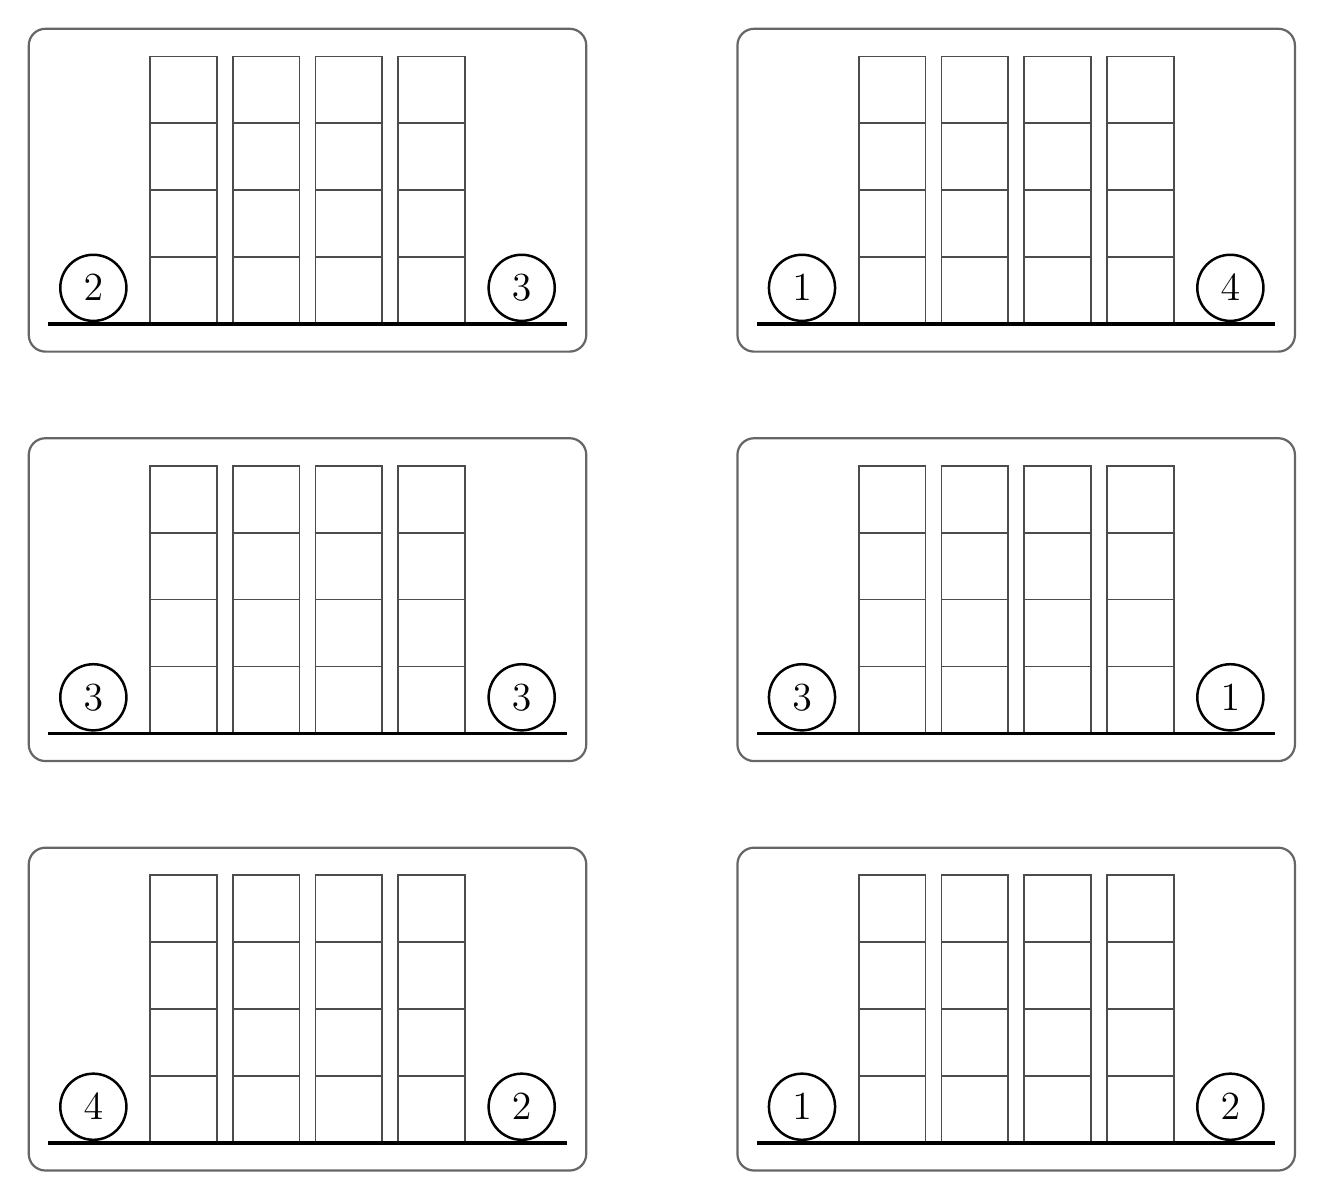
\begin{tikzpicture}
\begin{scope}[shift={(0.000,0.000)}]
\draw[line width=0.6pt, black!70] (0.000,0.000) rectangle (0.850,0.850);
\draw[line width=0.6pt, black!70] (0.000,0.850) rectangle (0.850,1.700);
\draw[line width=0.6pt, black!70] (0.000,1.700) rectangle (0.850,2.550);
\draw[line width=0.6pt, black!70] (0.000,2.550) rectangle (0.850,3.400);
\draw[line width=0.6pt, black!70] (1.050,0.000) rectangle (1.900,0.850);
\draw[line width=0.6pt, black!70] (1.050,0.850) rectangle (1.900,1.700);
\draw[line width=0.6pt, black!70] (1.050,1.700) rectangle (1.900,2.550);
\draw[line width=0.6pt, black!70] (1.050,2.550) rectangle (1.900,3.400);
\draw[line width=0.6pt, black!70] (2.100,0.000) rectangle (2.950,0.850);
\draw[line width=0.6pt, black!70] (2.100,0.850) rectangle (2.950,1.700);
\draw[line width=0.6pt, black!70] (2.100,1.700) rectangle (2.950,2.550);
\draw[line width=0.6pt, black!70] (2.100,2.550) rectangle (2.950,3.400);
\draw[line width=0.6pt, black!70] (3.150,0.000) rectangle (4.000,0.850);
\draw[line width=0.6pt, black!70] (3.150,0.850) rectangle (4.000,1.700);
\draw[line width=0.6pt, black!70] (3.150,1.700) rectangle (4.000,2.550);
\draw[line width=0.6pt, black!70] (3.150,2.550) rectangle (4.000,3.400);
\draw[line width=1.2pt] (-1.290,0) -- (5.290,0);
\draw[line width=0.9pt] (-0.720,0.460) circle (0.420);
\node at (-0.720,0.460) {\Large 2};
\draw[line width=0.9pt] (4.720,0.460) circle (0.420);
\node at (4.720,0.460) {\Large 3};
\draw[rounded corners=6pt, line width=0.8pt, black!60] (-1.540,-0.35) rectangle (5.540,3.750);
\end{scope}
\begin{scope}[shift={(9.000,0.000)}]
\draw[line width=0.6pt, black!70] (0.000,0.000) rectangle (0.850,0.850);
\draw[line width=0.6pt, black!70] (0.000,0.850) rectangle (0.850,1.700);
\draw[line width=0.6pt, black!70] (0.000,1.700) rectangle (0.850,2.550);
\draw[line width=0.6pt, black!70] (0.000,2.550) rectangle (0.850,3.400);
\draw[line width=0.6pt, black!70] (1.050,0.000) rectangle (1.900,0.850);
\draw[line width=0.6pt, black!70] (1.050,0.850) rectangle (1.900,1.700);
\draw[line width=0.6pt, black!70] (1.050,1.700) rectangle (1.900,2.550);
\draw[line width=0.6pt, black!70] (1.050,2.550) rectangle (1.900,3.400);
\draw[line width=0.6pt, black!70] (2.100,0.000) rectangle (2.950,0.850);
\draw[line width=0.6pt, black!70] (2.100,0.850) rectangle (2.950,1.700);
\draw[line width=0.6pt, black!70] (2.100,1.700) rectangle (2.950,2.550);
\draw[line width=0.6pt, black!70] (2.100,2.550) rectangle (2.950,3.400);
\draw[line width=0.6pt, black!70] (3.150,0.000) rectangle (4.000,0.850);
\draw[line width=0.6pt, black!70] (3.150,0.850) rectangle (4.000,1.700);
\draw[line width=0.6pt, black!70] (3.150,1.700) rectangle (4.000,2.550);
\draw[line width=0.6pt, black!70] (3.150,2.550) rectangle (4.000,3.400);
\draw[line width=1.2pt] (-1.290,0) -- (5.290,0);
\draw[line width=0.9pt] (-0.720,0.460) circle (0.420);
\node at (-0.720,0.460) {\Large 1};
\draw[line width=0.9pt] (4.720,0.460) circle (0.420);
\node at (4.720,0.460) {\Large 4};
\draw[rounded corners=6pt, line width=0.8pt, black!60] (-1.540,-0.35) rectangle (5.540,3.750);
\end{scope}
\begin{scope}[shift={(0.000,-5.200)}]
\draw[line width=0.6pt, black!70] (0.000,0.000) rectangle (0.850,0.850);
\draw[line width=0.6pt, black!70] (0.000,0.850) rectangle (0.850,1.700);
\draw[line width=0.6pt, black!70] (0.000,1.700) rectangle (0.850,2.550);
\draw[line width=0.6pt, black!70] (0.000,2.550) rectangle (0.850,3.400);
\draw[line width=0.6pt, black!70] (1.050,0.000) rectangle (1.900,0.850);
\draw[line width=0.6pt, black!70] (1.050,0.850) rectangle (1.900,1.700);
\draw[line width=0.6pt, black!70] (1.050,1.700) rectangle (1.900,2.550);
\draw[line width=0.6pt, black!70] (1.050,2.550) rectangle (1.900,3.400);
\draw[line width=0.6pt, black!70] (2.100,0.000) rectangle (2.950,0.850);
\draw[line width=0.6pt, black!70] (2.100,0.850) rectangle (2.950,1.700);
\draw[line width=0.6pt, black!70] (2.100,1.700) rectangle (2.950,2.550);
\draw[line width=0.6pt, black!70] (2.100,2.550) rectangle (2.950,3.400);
\draw[line width=0.6pt, black!70] (3.150,0.000) rectangle (4.000,0.850);
\draw[line width=0.6pt, black!70] (3.150,0.850) rectangle (4.000,1.700);
\draw[line width=0.6pt, black!70] (3.150,1.700) rectangle (4.000,2.550);
\draw[line width=0.6pt, black!70] (3.150,2.550) rectangle (4.000,3.400);
\draw[line width=1.2pt] (-1.290,0) -- (5.290,0);
\draw[line width=0.9pt] (-0.720,0.460) circle (0.420);
\node at (-0.720,0.460) {\Large 3};
\draw[line width=0.9pt] (4.720,0.460) circle (0.420);
\node at (4.720,0.460) {\Large 3};
\draw[rounded corners=6pt, line width=0.8pt, black!60] (-1.540,-0.35) rectangle (5.540,3.750);
\end{scope}
\begin{scope}[shift={(9.000,-5.200)}]
\draw[line width=0.6pt, black!70] (0.000,0.000) rectangle (0.850,0.850);
\draw[line width=0.6pt, black!70] (0.000,0.850) rectangle (0.850,1.700);
\draw[line width=0.6pt, black!70] (0.000,1.700) rectangle (0.850,2.550);
\draw[line width=0.6pt, black!70] (0.000,2.550) rectangle (0.850,3.400);
\draw[line width=0.6pt, black!70] (1.050,0.000) rectangle (1.900,0.850);
\draw[line width=0.6pt, black!70] (1.050,0.850) rectangle (1.900,1.700);
\draw[line width=0.6pt, black!70] (1.050,1.700) rectangle (1.900,2.550);
\draw[line width=0.6pt, black!70] (1.050,2.550) rectangle (1.900,3.400);
\draw[line width=0.6pt, black!70] (2.100,0.000) rectangle (2.950,0.850);
\draw[line width=0.6pt, black!70] (2.100,0.850) rectangle (2.950,1.700);
\draw[line width=0.6pt, black!70] (2.100,1.700) rectangle (2.950,2.550);
\draw[line width=0.6pt, black!70] (2.100,2.550) rectangle (2.950,3.400);
\draw[line width=0.6pt, black!70] (3.150,0.000) rectangle (4.000,0.850);
\draw[line width=0.6pt, black!70] (3.150,0.850) rectangle (4.000,1.700);
\draw[line width=0.6pt, black!70] (3.150,1.700) rectangle (4.000,2.550);
\draw[line width=0.6pt, black!70] (3.150,2.550) rectangle (4.000,3.400);
\draw[line width=1.2pt] (-1.290,0) -- (5.290,0);
\draw[line width=0.9pt] (-0.720,0.460) circle (0.420);
\node at (-0.720,0.460) {\Large 3};
\draw[line width=0.9pt] (4.720,0.460) circle (0.420);
\node at (4.720,0.460) {\Large 1};
\draw[rounded corners=6pt, line width=0.8pt, black!60] (-1.540,-0.35) rectangle (5.540,3.750);
\end{scope}
\begin{scope}[shift={(0.000,-10.400)}]
\draw[line width=0.6pt, black!70] (0.000,0.000) rectangle (0.850,0.850);
\draw[line width=0.6pt, black!70] (0.000,0.850) rectangle (0.850,1.700);
\draw[line width=0.6pt, black!70] (0.000,1.700) rectangle (0.850,2.550);
\draw[line width=0.6pt, black!70] (0.000,2.550) rectangle (0.850,3.400);
\draw[line width=0.6pt, black!70] (1.050,0.000) rectangle (1.900,0.850);
\draw[line width=0.6pt, black!70] (1.050,0.850) rectangle (1.900,1.700);
\draw[line width=0.6pt, black!70] (1.050,1.700) rectangle (1.900,2.550);
\draw[line width=0.6pt, black!70] (1.050,2.550) rectangle (1.900,3.400);
\draw[line width=0.6pt, black!70] (2.100,0.000) rectangle (2.950,0.850);
\draw[line width=0.6pt, black!70] (2.100,0.850) rectangle (2.950,1.700);
\draw[line width=0.6pt, black!70] (2.100,1.700) rectangle (2.950,2.550);
\draw[line width=0.6pt, black!70] (2.100,2.550) rectangle (2.950,3.400);
\draw[line width=0.6pt, black!70] (3.150,0.000) rectangle (4.000,0.850);
\draw[line width=0.6pt, black!70] (3.150,0.850) rectangle (4.000,1.700);
\draw[line width=0.6pt, black!70] (3.150,1.700) rectangle (4.000,2.550);
\draw[line width=0.6pt, black!70] (3.150,2.550) rectangle (4.000,3.400);
\draw[line width=1.2pt] (-1.290,0) -- (5.290,0);
\draw[line width=0.9pt] (-0.720,0.460) circle (0.420);
\node at (-0.720,0.460) {\Large 4};
\draw[line width=0.9pt] (4.720,0.460) circle (0.420);
\node at (4.720,0.460) {\Large 2};
\draw[rounded corners=6pt, line width=0.8pt, black!60] (-1.540,-0.35) rectangle (5.540,3.750);
\end{scope}
\begin{scope}[shift={(9.000,-10.400)}]
\draw[line width=0.6pt, black!70] (0.000,0.000) rectangle (0.850,0.850);
\draw[line width=0.6pt, black!70] (0.000,0.850) rectangle (0.850,1.700);
\draw[line width=0.6pt, black!70] (0.000,1.700) rectangle (0.850,2.550);
\draw[line width=0.6pt, black!70] (0.000,2.550) rectangle (0.850,3.400);
\draw[line width=0.6pt, black!70] (1.050,0.000) rectangle (1.900,0.850);
\draw[line width=0.6pt, black!70] (1.050,0.850) rectangle (1.900,1.700);
\draw[line width=0.6pt, black!70] (1.050,1.700) rectangle (1.900,2.550);
\draw[line width=0.6pt, black!70] (1.050,2.550) rectangle (1.900,3.400);
\draw[line width=0.6pt, black!70] (2.100,0.000) rectangle (2.950,0.850);
\draw[line width=0.6pt, black!70] (2.100,0.850) rectangle (2.950,1.700);
\draw[line width=0.6pt, black!70] (2.100,1.700) rectangle (2.950,2.550);
\draw[line width=0.6pt, black!70] (2.100,2.550) rectangle (2.950,3.400);
\draw[line width=0.6pt, black!70] (3.150,0.000) rectangle (4.000,0.850);
\draw[line width=0.6pt, black!70] (3.150,0.850) rectangle (4.000,1.700);
\draw[line width=0.6pt, black!70] (3.150,1.700) rectangle (4.000,2.550);
\draw[line width=0.6pt, black!70] (3.150,2.550) rectangle (4.000,3.400);
\draw[line width=1.2pt] (-1.290,0) -- (5.290,0);
\draw[line width=0.9pt] (-0.720,0.460) circle (0.420);
\node at (-0.720,0.460) {\Large 1};
\draw[line width=0.9pt] (4.720,0.460) circle (0.420);
\node at (4.720,0.460) {\Large 2};
\draw[rounded corners=6pt, line width=0.8pt, black!60] (-1.540,-0.35) rectangle (5.540,3.750);
\end{scope}
\end{tikzpicture}
\end{center}
\end{minipage}
\par\vspace{0.75cm}
\end{document}
